\documentclass[12pt, a4paper]{report}
\usepackage{graphicx}

\begin{document}

\begin{titlepage}
    \begin{center}
        \vspace*{4cm}
        
        % University Logo (replace with your university's logo)
        \includegraphics[width=0.2\textwidth]{}
         \begin{figure}
            \centering
            
\includegraphics[width=0.5\linewidth]{IIT-Delhi-Indian-Institute-of-Technology-Delhi.png}
            \begin{center}
                \textbf{DEPARTMENT OF MATHEMATICS}\\
                \textbf{INDIAN INSTITUTE OF TECHNOLOGY DELHI}
            \end{center}
            
            %\label{fig:enter-label}
        \end{figure}
        
        %\vspace{2cm}
        
        % Thesis Title
        \textbf{\Large VARIATIONAL ITERATION METHOD AND IT'S APPLICATIONS}
        
        \vspace{5.0cm}
        
        % Your Name
        \textbf {\Large Guguloth Ajay Kumar}
        
        

        % Your Degree
        %A thesis submitted in partial fulfillment of the requirements for the degree of (B.Tech +M.Tech)
        % Your Department
        %in the Department of Mathematics and Computing.
        
        %\vspace{0.1cm}
        
        % Your University Name and Year
        %\textbf{\Large JULY, 2024}
        
    \end{center}
\end{titlepage}
    
\end{titlepage}

\newpage

\begin{center}
    \Large
    VARIATIONAL ITERATION METHOD AND IT'S APPLICATIONS
    \vspace{1cm}
    
    \Large
    by
    
    \vspace{2cm}
    
    \Large
    GUGULOTH AJAY KUMAR
    
    \vspace{2cm}
    
    \Large
    Department of Mathematics
    
    \vspace{2cm}
    
    \Large
    Submitted
    
    \vspace{0.5cm}
    
    \large
    in fulfillment of the requirements for the degree of (B.Tech + M.Tech).
    
    \vspace{1.5cm}
    
    \Large
    to the
    
    \vspace{1.5cm}
    
    \Large
    Indian Institute of Technology Delhi
    
    \vspace{1cm}
    
    \Large
    July  2024
\end{center}

\clearpage

% Certificate
\chapter*{Certificate}
\addcontentsline{toc}{chapter}{Certificate}
This is to certify that the thesis entitled \textit{Variational Iteration Method and It's Applications} submitted by Mr. Guguloth Ajay Kumar to the Indian Institute of Technology Delhi, for the award of the Degree of Master's Degree, is a record of the original bonafide thesis work carried out by his under my supervision. The thesis has reached the standards fulfilling the requirements of the regulations relating to the degree. The results contained in this thesis have not been submitted in part or full to any other university or institute for award of any degree or diploma.

\vspace{1in}
\begin{flushright}
    Konijeti Sreenadh\\
    Professor\\
    Department of Mathematics\\
    Indian Institute of Technology Delhi\\
    New Delhi-110 016
\end{flushright}
\begin{flushleft}
    New Delhi\\
    July 2024
\end{flushleft}

% Acknowledgements
\chapter*{Acknowledgements}
\addcontentsline{toc}{chapter}{Acknowledgements}
To pursue a career in academics needs perseverance in learning and a mind that is always open for new ideas. My journey as a M.Tech student has taught me the value of endurance and continuance with positive approach. Completing M.Tech from a renowned institute like Indian Institute of Technology Delhi is the life changing milestone in my career. I am indebted and grateful to many people and institutions for my achievement \vspace{0.5cm}.

First and foremost, I am much obliged to my thesis supervisor Prof. Konijeti Sreenadh. I am extremely blessed to have such an encouraging and helpful supervisor who taught me the essence of doing this work. Prof. Sreenadh amazingly eased my journey with his awareness, recognition and understanding of the flourishing research areas. His aptness in anticipating my academic as well as non-academic vacillations and ups and downs always kept me proceeding in the right direction. His knowledge, passion, motivation and patience were the crucial element in accomplishment of this thesis.I sincerely acknowledge the efforts of the examiners/reviewers. It has greatly helped in improving the thesis \vspace{0.5cm}.

I am immensely indebted to my Parents for their unending support, encouragement and patience. No words can express my gratitude towards them. My special appreciation goes to my brothers (Praveen) and (Vinay) for their affection, assistance and sacrifices \vspace{0.5cm}.

Above all I am eternally indebted to God for graciously bestowing his blessings and making this happen \vspace{0.5cm}.

\begin{flushright}
    New Delhi\\
    Guguloth Ajay Kumar
\end{flushright}



\chapter*{Notations}
\addcontentsline{toc}{chapter}{Notations}
\begin{tabbing}
    \hspace{2in} \= \kill
    $a_1, a_2, a_3, R$ \> coefficients \\
    $f(x, t)$ \> forcing function \\
    $q(x, t)$ \> forcing function \\
    $u_0(x, t)$ \> initial approximation \\
    $\mathcal{L}\{f(t)\}$ \> Laplace transform \\
    $\mathcal{L}^{-1}\{F(s)\}$ \> inverse Laplace transform \\
    $|| \cdot ||$ \> norm \\
    $E_j(t)$ \> series approximation \\
    $u_{tt} = u_{xx}$ \> wave equation \\
    $u_{n+1}(x, t)$ \> correction functional \\
     $\|.\|$ \> norm when domain is obvious, or of no particular significance \\
    $v_i$ \> $v(x_i)$ \\
    $C, C_s, s = 0, 1, \ldots$ \> generic positive constants, independent of $M, N$ \\
    % Additional Notations
    $E_{\alpha,\beta}(u)$ \> Mittag-Leffler function \\
    $\frac{\partial^\alpha u}{\partial x^\alpha}$ \> partial fractional derivative with respect to $x$ \\
    $\frac{\partial^\beta u}{\partial t^\beta}$ \> partial fractional derivative with respect to $t$ \\
    $\frac{\partial^\gamma u}{\partial t^\gamma}$ \> partial fractional derivative with respect to $t$ \\
    $J^\alpha$ \> Riemann-Liouville fractional integral \\
    $J^\beta$ \> Riemann-Liouville fractional integral \\
    $D^\alpha_t$ \> Riemann-Liouville fractional derivative \\
    $D^\alpha_t$ \> Caputo time fractional derivative \\
    $\Gamma(z)$ \> Gamma function \\
    $\frac{\partial^\alpha u(x,t)}{\partial t^\alpha}$ \> general time fractional differential equation \\
    $u(x, t)$ \> function of time and space \\
    $S$ \> asset price \\
    $S_0$ \> initial asset price \\
    $\tau, t$ \> time variables \\
    $C$ \> call option price \\
    $P$ \> put option price \\
    $\sigma$ \> market volatility \\
    $r$ \> risk free interest rate \\
    $D$ \> dividend yield \\
    $K$ \> strike price \\
    $T$ \> maturity time of the contract \\
    $W$ \> Wiener process \\
    $\epsilon$ \> small parameter \\
\end{tabbing}




\clearpage
%\begin{document}
%\maketitle
%\maketitle CONTENTS
\begin{center}
\textbf{\Large Abstract}
\end{center}
The project aims to study a new kind of analytical technique for a non-linear problem called the Variational Iteration Method (VIM), which is described and used to give approximate solutions for some well-known Non-Linear problems.\\

It is a modification of the General Lagrange Multiplier Method. In this method, the problems are initially approximated with possible unknowns. Then a correction functional is constructed by a general lagrange multiplier, which can be identified optimally via a variational theory.\\

The VIM is used to solve effectively, easily, and accurately a large class of non-linear problems with approximations which converge rapidly to accurate solutions. For linear problems, its exact solution can be obtained by only one iteration step due to the fact that the Lagrange multiplier can be exactly identified.\\

In chapter 3, the variational iteration method is applied to solve integral differential equations. Some examples are given to illustrate the effectiveness of the method.\\

In chapter 4, Laplace variational iteration strategy, based on the (VIM) and Laplace transform, is presented for the exact/numerical solution of linear and nonlinear differential equations.\\

In chapter 5, VIM is applied to different types of fractional differential equations. Also, the Laplace transform is used to solve certain classes of fractional differential equations.

\clearpage

\begin{singlespace}
\tableofcontents
\thispagestyle{empty}

%\listoftables
%\addcontentsline{toc}{chapter}{LIST OF TABLES}
%\listoffigures
%\addcontentsline{toc}{chapter}{LIST OF FIGURES}
\end{singlespace}
\clearpage



%\documentclass{article}

%\begin{document}

%This is some text above the horizontal lines.

\bigskip % Add some vertical space

\rule{\textwidth}{1.4pt} % First horizontal line

\bigskip % Add some vertical space

\chapter{\textbf{\LARGE Variational Iteration Method}}

\bigskip % Add some vertical space

\rule{\textwidth}{1.4pt} % Second horizontal line

\bigskip % Add some vertical space

%This is some text below the horizontal lines.

%\end{document}

   \section{Introduction} 
     \vspace{4.5pt}
     The Variational Iteration Method (VIM) was first developed by Chinese mathematician Ji-Huan He, professor at Donghua University. The VIM was initially proposed toward the end of the most recent century and completely grew in 2006 and 2007. 
    
    \vspace{4.5pt}
     
     This method is a modification of a General Lagrange Multiplier.Variational iteration method (VIM) is relatively new approaches to provide approximate solutions to linear and nonlinear problems.The variation method is an iterative method based on the use of general lagrange multiplier,restricted variation and correctional functional which has a wide application for the solutions of non linear ordinary and partial differential equation.
         \vspace{4.5pt}
         
     Differential equations are used in a various fields as Physics,Biology,Mathematics.In this paper we are going to learn how this method converge rapidly to accurate solution for Non-Linear Problem.

\section{VIM}
For a linear operator L, non-linear operator N and analytic function g(×), consider the equation
\begin{equation}
    Lu(x)+Nu(x) = g(x)
\end{equation}
Assuming $u_{0}(x)$ is the solution of Lu = 0,
     \begin{equation}
      u_{cor}(x_0) = u_0(x_0) + \int_{0}^{x_0} \lambda (Lu_0+Nu_0-g)\,dx
     \end{equation}
%\vspace{4.5pt}
where $\lambda$ is a general Lagrange multiplier which can be identified optimally via variational theory and $u_{cor}$ is the corrected solution at $x_0$. The above (2) is modified into an iteration method as following :
     \begin{equation}
            u_{n+1}(x_0) = u_n(x_0) + \int_{0}^{x_0} \lambda(s) [Lu_n(s)+N\tilde{u}_n(s)-g(s)]\,ds
     \end{equation}
with $u_0(x)$ is an initial approximation with possible unknowns and $\tilde{u}\_n$ considered as a restricted variation i.e. $\delta \tilde{u}_n=0 $ ,$u_n$ denotes the n'th approximation.As $x_0$ is arbitrary,we can rewrite the equation as:

     \begin{equation}
            u_{n+1}(x) = u_n(x) + \int_{0}^{x} \lambda(s) [Lu_n(s)+N\tilde{u}_n(s)-g(s)]\,ds
     \end{equation}
The above modified method called Variational Iteration Method solves non-linear problems effectively, easily and accurately with approximations converging to accurate solutions. In this method, we obtain a series which converges fast to the exact solution.
\section{Procedure of Solving Equations}
Let's consider a general equation,
\begin{equation}
    Lu(x) +Nu(x) = g(x).
\end{equation}
here L represents the Linear operator,N represents the Non-linear operator and g represents Inhomogenous function.Procedure of solving these equations
\begin{itemize}
    \item step 1:For solving the equation by Variational Iteration Method,the correctional functional is 
    \begin{equation}
        u_{n+1}(x) = u_n(x) + \int_{0}^{x} \lambda(\xi) [Lu_n(\xi)+N\tilde{u}_n(\xi)-g(\xi)]\,d\xi
    \end{equation}
    
    \item step 2:$\lambda$ is obtained by applying integration by parts in (6),taking $\delta \tilde{u}_{n+1}=0$ and comparing terms on both sides.

    
    \item step 3:Choose initial approximation $u_0 $,usually depending on intitial conditions given in problem.And now find successive approximations $u_n(x)$, $n > 0$.

   
    \item step 4:Taking $lim_{n\to\infty}$,we get the exact solution as u(x) = $ l  i  m_{n\to\infty}$$ u_n(x)$

    
\end{itemize}

\textbf{Remark 1:}We can also choose Initial approximation to be the solution of homogenous equation with given initial condition. Initial approrimations can also be chosen with unknown parameters which can be found using given initial conditions in problem.

\textbf{Remark 2:}For linear problems, its exact solution can be obtained by only one iteration due to the fact that the Lagrange multiplier can be exactly identified. For nonlinear equation, the Lagrange multiplier is difficult to be identified. To overcome the difficulty, we apply restricted variations to nonlinear terms. But the restricted variations are applied only to non-linear terms, and the lesser the application of restricted variations, the faster the approximations converges to its exact solution.

\textbf{Example : 1} Now, consider an example of Ordinary Differential Equation
\begin{equation}
    u''(t) +w^2 u(t) = 0, 
    u(0)=1 , u'(0)= 0
\end{equation}
\textbf{Solution :}By solving the problem with VIM,The correctiona functional is given by
\begin{equation}
    u_{n+1}(t) = u_n(t) + \int_{0}^{t} \lambda(s) [d^2u_n(s)/ds^2+w^2 \tilde{u}_n(s)]\,ds
\end{equation}
For finding $\lambda$, making the above correction functional stationary using $\delta \tilde{u}_{n}=0$ above equation,
%\usepackage{amsmath}
\begin{align*}
    
    \delta u_{n+1} (t) & = \delta  u_{n} (t) +  \delta  \int_0^t  \lambda (s) [u''_n (s) + w^2 \tilde{u}_n(s)](ds) \\
    
    & = \delta u_{n} (t) + \lambda (s)\delta u'_{n} (s)\bigg|_0^t - \int_0^t \lambda(s) \delta u'_{n} (s) (ds) + \int_0^t \lambda(s) w^2 \delta \tilde{u}_n(s) ds \\
    
    & = \delta u_{n} (t) + \lambda (s)\delta u'_{n} (s)\bigg|_{s=t} + \lambda '(s) \delta u_{n} (s) \bigg|_{s=t} + \int_0^t \lambda''(s) \delta u_{n} (s) (ds) + 0
\end{align*}



\vspace{3.5pt}

So ,$\delta \tilde{u}_{n+1}(s) = 0 $ gives the following stationary conditions,

\vspace{3.5pt}
%\documentclass{article}

%\begin{document}
\[
\begin{array}{ll}
    \delta u_{n}(s) : & \lambda''(s) = 0 , \\
    
    \delta u_{n}(s) : & 1 - \lambda'(s)\bigg|_{s=t} = 0 , \\
    
    \delta u'_{n}(s) : & \lambda(s)\bigg|_{s=t} = 0.
\end{array}
\]
%\end{document}
\vspace{3.5pt}

Solving the above equations we get , $\lambda (s) = s-t $.
\vspace{4.5pt}

Now substitute the $\lambda (s)$ value in correction functional (8),

\begin{equation}
    u_{n+1}(t) = u_n(t) + \int_{0}^{t} (s-t) [d^2u_n(s)/ds^2+w^2 \tilde{u}_n(s)]\,ds
\end{equation}

Choosing Initial approximation, $u_{0}(t)$= 1 . 
\vspace{2.5pt}
Therefore, the successive approximations are,

\begin{center}
    $u_{1}(t) = 1 - \frac{1}{2!} (w^2t^2)$ \\
    
    $u_{2}(t) = 1 - \frac{1}{2!} (w^2t^2) + \frac{1}{4!}(w^4 t^4)$ \\
    . \\
    
    . \\
    
    . \\
    
    . \\
    
    $u_{n}(t) = 1 - \frac{1}{2!}w^2 t^2 + \frac{1}{4!}(w^4 t^4) + \ldots + (-1)^n \frac{1}{(2n)!} (w^{2n} t^{2n})$
\end{center}

\vspace{4.5pt}
Therefore,the exact solution is ,
\[
u(t) = \lim_{{n \to \infty}} u_n(t)
\]
\[
= coswt .
\]

\section{Convergence Analysis}
The variational iteration method changes the differential equation to a recurrence sequence of functions. The limit of that sequence is considered as the solution of the partial differential equation. Using the VIM,it is possible to find the exact solution or an approximate solution of the problem. Now,our emphasis will be on the converegence of the Variational Iteration Method.

{\textbf{Theorem 1.}} Let the equation be,
\begin{center}
              $Lu_{n}(t) + Nu_{n}(t) = g(t)$
\end{center}
and A ,defined as 
\begin{equation}
A[u] = \int_0^t -\frac{1}{(m-1)!} (s-t)^{m-1} [Lu_{n}(s) + Nu_{n}(s) - g(s)] \, ds
\end{equation}

be an operator from a Hilbert Space H to H. The series solution ,
\begin{center}
%    \begin{equation}
      $u(t) = \sum_{k=0}^{\infty} v_k(t)$
%\end{equation}
\end{center}

\begin{align}
v_k(t) &= A[v_o+v_1+v_2+\dots+v_k], \\
\textit{converges if} $ \exists (0 < \gamma < 1) $ \text{ s.t.}
\end{align}


\begin{center}
    $||A [V_0+V_1+V_2+......+V_{k+1} ] || \leq  \gamma ||A [V_0+V_1+V_2+......+V_{k} ] || $   
\end{center}
(i.e $||v_{k+1}|| \leq \gamma ||v_{k}|| $

\vspace{9pt}
\clearpage
\textbf{Proof :} Define the sequence of partial sums $\{S_n\}_{n=0}^\infty $


\begin{center}
     $ S_0= v_0, $ \\
     $S_1 = v_0 +v_1 $, \\
     $S_2 = v_0 +v_1+v_2$
     . \\
    
     . \\
    
     . \\
     
     . \\
    $ S_n = v_0 +v_1 +v_2+.......+v_n $\\
     
\end{center}
    
Now ,We show that $\{S_n\}_{n=0}^\infty $ is a Cauchy Sequence in the Hilbert Space H.
\vspace{9pt}
Consider,
\vspace{5pt}

$||S_{n+1}-S_n|| = ||v_{n+1}|| \leq \gamma ||v_n|| \leq \gamma ^2 ||v_{n-1}|| \leq .......\leq \gamma^{n+1} ||v_0|| $ \\

For every n,m $>$ 0 and n $\geq m$ we have,

\begin{align*}
    
  
    
    $ ||S_n - S_m|| $ & = $||(S_n - S_{n-1}) +(S_{n-1}-S_{n-2}) +....+ (S_{m+1}- S_m ) $ 
    
    &  \leq ||(S_n - S_{n-1})|| +||(S_{n-1}-S_{n-2})|| +....+ ||(S_{m+1}- S_m )|| \\ 
    
    & \leq \gamma^n ||v_0|| + \gamma^{n-1}||v_0||+....+\gamma^{m+1} ||v_0|| \\ 

    
    &= \left(\frac{1 - \gamma^{n-m}}{1 - \gamma}\right) \gamma^{m+1} ||v_0|| \\

    
\end{align*}



since $0 \leq \gamma \leq 1$ we get ,
\vspace{9pt}

\begin{center}
    $\lim_{{n,m \to \infty}} \|S_n - S_m\| = 0 $
\end{center}

 Therefore, $\{S_n\}_{n=0}^\infty $ is a Cauchy Sequence in the Hilbert Space H and hence, the series solution 
 $u(t) = \sum_{k=0}^{\infty} v_k(t)$  converges.
\clearpage
\textbf{Theorem 2. }If the series Solution  
\begin{center}
    $u(t) = \sum_{k=0}^{\infty} v_k(t)$
\end{center} is converges ,then it is an exact solution of a Non-linear equation
\begin{center}
    Lu(t) +Nu(t) = g(t) .
\end{center}

\textbf{Proof:} Suppose the series solution converges, say
\begin{center}
    $ \phi(t) = \sum_{m=0}^{\infty} v_m(t)$
\end{center}
then we have , 
\begin{center}
    $\lim_{{m \to \infty}} v_m = 0 , $ \\
    $\sum_{m=0}^n [v_{m+1} - v_m] = v_{n+1} - v_0$\\
\end{center}
and so, 
\begin{equation}
    \sum_{m=0}^n [v_{m+1} - v_m] = \lim_{{m \to \infty}} v_m - v_0 = - v_0 
\end{equation}
Applying the operator Laplace operator 'L' to both sides of (11) then we have 
\begin{center}
    $ \sum_{m=0}^n L [v_{m+1} - v_m] = -L[v_0] = 0 $
\end{center}
Also we have , 
%\vspace{9pt}
\begin{center}
    $L[v_{m+1}-v_m] = L[A[v_0+v_1+v_2+.....+v_m] - A[v_0+v_1+v_2+.....+v_{m-1}]]$ \\
\end{center}

when $m \geq 1 $, then by (Eq..10)

\begin{center}

   L[v_{m+1} - v_m]    = L\biggl[\int_0^t & \frac{(-1)^m}{(m-1)!} (s- 
   t)^{m-1} &\biggl( L[v_0 + v_1 + v_2 + \dots + v_m] \\
   $ - L[v_0 + v_1 + v_2 + \dots + v_{m-1}] + N[v_0 + v_1 + v_2 + \dots + &v_m] - N[v_0 + v_1 + \dots + v_{m-1}] \biggr) ds \biggr] \\$
   
\end{center}

then,
\begin{center}
    L[v_{m+1}-v_m] = L[v_m]+ + N[v_0 + v_1 + v_2 + \dots + &v_m] - N[v_0 + v_1 + \dots + v_{m-1}]
\end{center}

consequently, we have
\begin{center}
    \sum_{m=0}^n L [v_{m+1} - v_m] = &\quad L[v_0] + N[v_0] - g(t) \\
\end{center}
\begin{center} 
&\quad + L[v_1] + N[v_0 + v_1] - N[v_0] \\
&\quad + L[v_2] + N[v_0 + v_1 + v_2] - N[v_0 + v_1] \\
&\quad \vdots \\
&\quad + L[v_n] + N[v_0 + v_1 + v_2 + \ldots + v_n] - N[v_0 + v_1 + v_2 + \ldots + v_{n-1}]

\end{center}

Therefore, 
\begin{center}
    $\sum_{m=0}^{\infty} L [v_{m+1} - v_m] =  \sum_{m=0}^{\infty} L[v_m] + \sum_{m=0}^{\infty} N[v_m] - g(t) $
\end{center}
Since we have,
 \begin{center}
     $\sum_{m=0}^{\infty} L[v_{m+1}-v_m]= 0$
 \end{center}
 Then $\phi(t) = \sum_{m=0}^{\infty} v_m(t)$ is an exact Solution of the given problem.

\textbf{Remark 3:} A sufficient condition for convergence of VIM to the exact solution is that $ \exists (0 < \gamma < 1) $ \text{ s.t.}
%\end{align}

\begin{center}
    $||A [V_0+V_1+V_2+......+V_{k+1} ] || \leq  \gamma ||A [V_0+V_1+V_2+......+V_{k} ] || $   
\end{center}
\begin{center}
    (i.e $||v_{k+1}|| \leq \gamma ||v_{k}|| $
\end{center}
\clearpage
\textbf{Theorem 3.} If the truncated series 
\begin{center}
    $\sum_{k=0}^{\infty} v_k(t)$
\end{center}
is used as an approximation to the solution u(t) then the maximum error $E_j(t)$ is 
\begin{center}
    $E_j(t) \leq \Large{\frac{1}{1 - \gamma} \cdot \gamma^{j+1} \cdot \|v_0\|}$
\end{center}
\textbf{Proof.} From Theorem 1 we have, for  $n\geq m $
\begin{center}
    $||S_n - S_m || \leq \left(\frac{1 - \gamma^{n-m}}{1 - \gamma}\right) \gamma^{m+1} ||v_0|| $
\end{center}

Now as $n \to \infty$ then $S_n \to u(t) $ so,
\begin{center}
    $$||u(t) - \sum_{k=0}^{\infty} v_k(t)|| \leq \left(\frac{1 - \gamma^{n-m}}{1 - \gamma}\right) \gamma^{m+1} ||v_0|| $$
\end{center}
Also, since $(0 < \gamma < 1)$  we have $1 - \gamma^{n-m} < 1$ .Therefore,
\begin{center}
    $||u(t) - \sum_{k=0}^{\infty} v_k(t)|| \leq \Large{\frac{1}{1 - \gamma} \cdot \gamma^{m+1} \cdot \|v_0\|}$
\end{center}

\clearpage 


%\documentclass{article}

%\begin{document}

%This is some text above the horizontal lines.

\bigskip % Add some vertical space

\rule{\textwidth}{1.4pt} % First horizontal line

\bigskip % Add some vertical space

\chapter{\textbf{\LARGE Solution Approaches to ODE's and PDE's}}

\bigskip % Add some vertical space

\rule{\textwidth}{1.4pt} % Second horizontal line

\bigskip % Add some vertical space

%This is some text below the horizontal lines.

%\end{document}

\section{Introduction}
In this chapter,we will study some numerical examples of  the Ordinary differential equations,Partial differential equations and Scheme of solving System of differential equation by Variational Iteration Method.

\section{Solving Wave Equation in Unbounded Domain}
Now consider the following wave equation in 1-dimension and unbounded domain 
\begin{center}
    $u_{tt} = u_{xx}  ,  - \infty < x < \infty\\$
    $ & u(x, 0) = sinx , u_t(x, 0 ) = 0 $
\end{center}    

\textbf{Solution} Let the correction functional be 

\begin{center}
    $u_{n+1}(x,t) = u_n(x,t) + \int_{0}^{t} \lambda(s) \left[\frac{{\partial^2u_n(x,s)}}{{\partial s^2}} - \frac{{\partial^2\tilde{u}_n(x,s)}}{{\partial x^2}}\right] \ \partial s$
\end{center}

Using $\delta \tilde{u}_n=0 $ in above equation, we get Stationary conditions :
\[
\begin{array}{ll}
    \delta u_{n}(s) : & \lambda''(s) = 0 , \\
    
    \delta u_{n}(s) : & 1 - \lambda'(s)\bigg|_{s=t} = 0 , \\
    
    \delta u'_{n}(s) : & \lambda(s)\bigg|_{s=t} = 0.
\end{array}
\]
On solving we get 
\begin{center}
    $\lambda(s) = s-t .$
\end{center}
Choose ,Initial Approximation : $u_0(x,t) = sinx$.
\text{Therefore ,the correction functional is}
\begin{center}
    $u_{n+1}(x,t) = u_n(x,t) + \int_{0}^{t} (s-t) \left[\frac{{\partial^2u_n(x,s)}}{{\partial s^2}} - \frac{{\partial^2\tilde{u}_n(x,s)}}{{\partial x^2}}\right] \ \partial s$
\end{center}

Then the successive approximations are:
\begin{center}
    $u_1(x,t)  = sinx - \frac{t^2}{2!} sinx $ \\
    & $u_2(x,t) = sinx - \frac{t^2}{2!} sinx + \frac{t^4}{4!} sinx $ \\
    & $u_3(x,t) = sinx - \frac{t^2}{2!} sinx + \frac{t^4}{4!} sinx - \frac{t^6}{6!}sinx $ \\
    & .\\
    & . \\
    & . \\

    & $u_n(x,t) = sinx\large[ 1 - \frac{t^2}{2!} + \frac{t^4}{4!}- \frac{t^6}{6!} + ......]$
\end{center}
Therefore the exact solution is,
\begin{center}
    $u(x,t) =\lim_{{n \to \infty}} u_n(x, t) = sinx cos t$
\end{center}

\section{Comparison}
Here we are comparing the exact solution and numerical approximations of a problem by Variational iteration method. Consider the following equation

\begin{center}
    $u''(t) - 2e^{u(t)} = 0 , 0<t<1 $ \\
    & $u(0) = 0 , u'(0) = 0$ \\
\end{center}
Solving by VIM correction functional is , 
\begin{center}
    $u_{n+1}(t) = u_n(t) + \int_{0}^{t} \lambda(s)\left  [\frac{{d^2u_n(s)}}{{ds^2}} - 2 e^{\tilde u_n(s)}\right ]  ds$
\end{center}
By above procedure (in previous example),solving for $\lambda $ \\
we get , $\lambda(s) = (s-t)$ \\
Choosing $u_0 = 0$ \\
Then, $u_1=t^2$ \\

Now we take the first approximations obtained by VIM as a solution of the given problem. And the exact solution of the given problem is 
\begin{center}
    u(t) = -2 ln(cos x)
\end{center}
 In the below table ,comparison between the exact solution and numerical solution obtained for u(t) of a 2-iterate VIM solution is shown for different points.

\begin{table}[ht]
\centering
\begin{tabular}{|c|c|c|c|}
\hline
t & Exact Sol & Approx.Sol by VIM & Absolute Error \\
\hline
0 & 0 & 0 & 0 \\
\hline
 0.1 & 0.010016711 & 0.01 & 0.000016711 \\
\hline
 0.2 & 0.040269546 & 0.04 &  0.000269546\\
\hline
 0.3 & 0.091383312 & 0.09 & 0.001383312 \\
\hline
 0.4 & 0.164458038 & 0.16 & 0.004458038  \\
\hline
\end{tabular}
%\caption{A 6x4 Table}
\label{tab:mytable}
\end{table}

\bigskip 
\bigskip 
\bigskip 

\begin{figure}
    \centering
    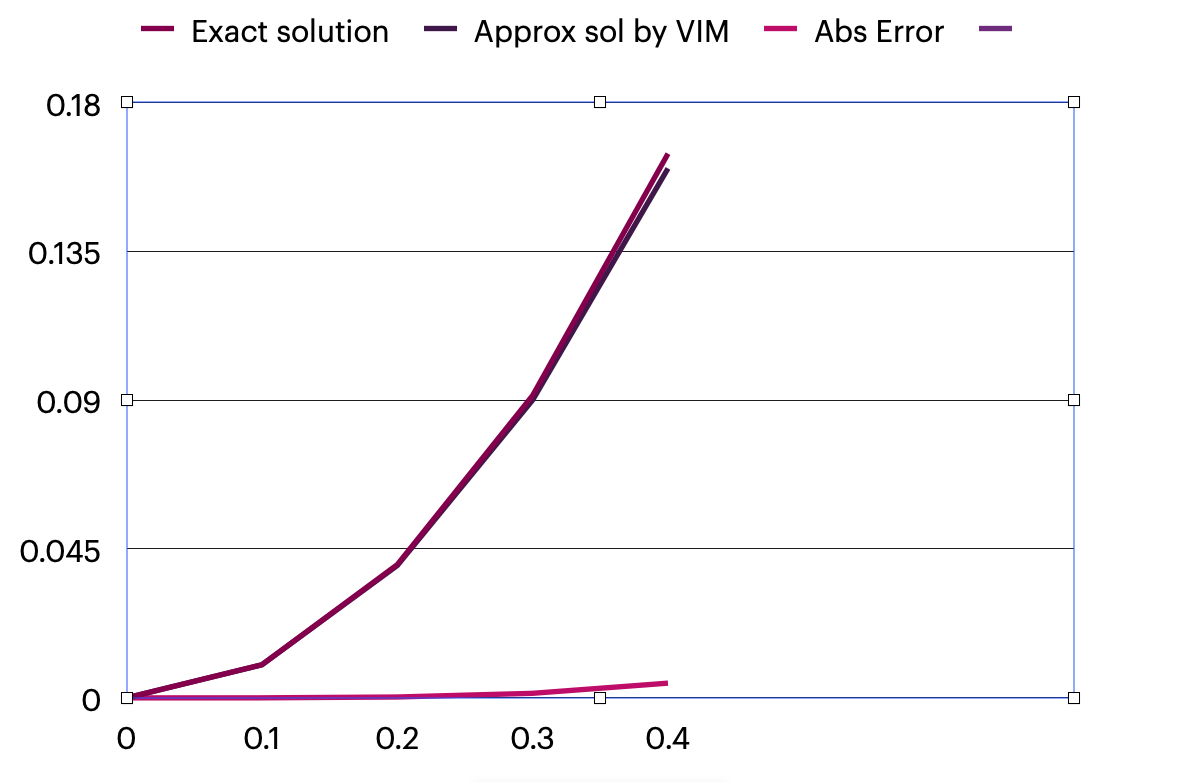
\includegraphics[width=0.5\linewidth]{Screenshot 2023-09-18 at 3.43.03 PM.png}
    \caption{}
    \label{fig:enter-label}
\end{figure}

In the above comparison, we are taking the first approximation as the solution by VIM  and we see that error is very small at starting time points, but if we calculate few more iterations by this method and calculate the error taking that to be exact solution ,then error will definitely decrease.So, we conclude that VIM is very efficient in finding the numerical solution of linear and non linear differential equation.

\section{System of differential equation}

Consider the m equations,
\begin{center}
    $L_1(y_1) + N_1(y_1,y_2,.....,y_m) = g_1(x) $ \\
    & $L_2(y_2) + N_2(y_1,y_2,.....,y_m) = g_2(x)$ \\
    & . \\
    & . \\
    & . \\
    & L_m(y_m) + N_m(y_1,y_2,.....,y_m) = g_m(x) \\
\end{center}
Where $L_i$ is linear w.r.t $y_i$ and $N_i$ is non linear part of i'th equation.

\textbf{} Using VIM, The correctional functionals are,
\begin{center}
    $y_{i(n+1)} = y_{in} + \int_{0}^{x} \lambda_i [L_i(y_{in}(s)) + N_i(\tilde y_{1n} (s),.....,\tilde y_{mn}(s)) - g_i(s)] ds $
\end{center}

Consider another correctional functional as 
\begin{center}
    $y_{i(n+1)} = y_{in} + \int_{0}^{x} \lambda_i [L_i(y_{in}(s)) + N_i(y_{1(n+1)}(s),...,y_{(i-1)(n+1)}(s), y_{1n} (s),...,y_{mn}(s)) - g_i(s)] ds$
\end{center}
for i = 2,...,m. 
\textbf{}In the correctional function above ,which is Corrected variational Iteration Method updated values $y_{1(n+1)},y_{2(n+1)}...,y_{(i-1)(n+1)} $ are used for finding $y_{i(n+1)}$.This accelerates the convergence of the system of sequences. Therefore, using just a few terms of the sequences, an accurate solution can be obtained for larger domain of the problem.It is especially useful when computing more terms of the sequences is difficult or Impossible.



\textbf{\Large Example }
$$
\begin{array}{ll}
\frac{d x}{d t}=x+3 y-3 e^2 t, & x(0)=1 \\
\frac{d y}{d t}=4 x+2 y+4 e^t, & y(0)=1
\end{array}
$$

Solution :
We know the exact solution of the system is,
$$
\begin{aligned}
& x(t)=e^t \\
& y(t)=e^{2 t}
\end{aligned}
$$

Using VIM the correctional functionals are,
$$
\begin{aligned}
& x_{n+1}=x_n-\int_0^t\left[x_n^{\prime}-x_n-3 y_n+3 e^{2 s}\right] d s, \\
& y_{n+1}=y_n-\int_0^t\left[y_n^{\prime}-4 x_n-2 y_n-4 e^s\right] d s
\end{aligned}
$$

Choosing initial approximations for VIM, $x_0=1, y_0=1$
Using (2.1) the correctional functionals are,
$$
\begin{aligned}
& \bar{x}_{n+1}=\bar{x}_n-\int_0^t\left[\bar{x}_n^{\prime}-\bar{x}_n-3 \bar{y}_n+3 e^{2 s}\right] d s, \\
& \bar{y}_{n+1}=\bar{y}_n-\int_0^t\left[\bar{y}_n^{\prime}-4 \bar{x}_{n+1}-2 \bar{y}_n-4 e^s\right] d s
\end{aligned}
$$

Choosing initial approximations for CVIM, $\bar{x}_0=1, \bar{y}_0=1$
\clearpage
In the table below, we calculate the error between the exact solution and the solutions obtained from VIM and CVIM.\\
We are taking the 10th approximations as the solutions of VIM and CVIM

\begin{table}[h!]
\centering
\begin{tabular}{|c|c|c|c|c|}
\hline
$t$ & $\left\|x(t)-x_{10}(t)\right\|$ & $\left\|x(t)-\bar{x}_{10}(t)\right\|$ & $\left\|y(t)-y_{10}(t)\right\|$ & $\left\|y(t)-\bar{y}_{10}(t)\right\|$ \\ \hline
0.1 & $0.3189 \times 10^{-11}$ & $0.2987 \times 10^{-14}$ & $0.4253 \times 10^{-11}$ & $0.1173 \times 10^{-14}$ \\ \hline
0.2 & $0.6625 \times 10^{-8}$ & $0.1072 \times 10^{-10}$ & $0.8834 \times 10^{-8}$ & $0.4741 \times 10^{-11}$ \\ \hline
0.3 & $0.5814 \times 10^{-6}$ & $0.1520 \times 10^{-8}$ & $0.7752 \times 10^{-6}$ & $0.7390 \times 10^{-9}$ \\ \hline
0.4 & $0.1396 \times 10^{-4}$ & $0.5618 \times 10^{-7}$ & $0.1862 \times 10^{-4}$ & $0.2956 \times 10^{-7}$ \\ \hline
0.5 & $0.1650 \times 10^{-3}$ & $0.9827 \times 10^{-6}$ & $0.2200 \times 10^{-3}$ & $0.5543 \times 10^{-6}$ \\ \hline
0.6 & $0.1244 \times 10^{-2}$ & $0.1064 \times 10^{-4}$ & $0.1659 \times 10^{-2}$ & $0.6385 \times 10^{-5}$ \\ \hline
0.7 & $0.6888 \times 10^{-2}$ & $0.8255 \times 10^{-4}$ & $0.9185 \times 10^{-2}$ & $0.5332 \times 10^{-4}$ \\ \hline
0.8 & $0.3039 \times 10^{-1}$ & $0.4996 \times 10^{-3}$ & $0.4052 \times 10^{-1}$ & $0.3330 \times 10^{-3}$ \\ \hline
0.9 & 0.1127 & $0.2498 \times 10^{-2}$ & 0.1503 & $0.1744 \times 10^{-2}$ \\ \hline
\end{tabular}
\caption{Comparison of Norms at Different Time Points}
\label{table:comparison_of_norms}
\end{table}



\clearpage


%\documentclass{article}

%\begin{document}

%This is some text above the horizontal lines.

\bigskip % Add some vertical space

\rule{\textwidth}{1.4pt} % First horizontal line

\bigskip % Add some vertical space

\chapter{\textbf{\LARGE Integral Differential Equations}}

\bigskip % Add some vertical space

\rule{\textwidth}{1.4pt} % Second horizontal line
\bigskip % Add some vertical space

\section{Introduction}
Various kind of analytical methods and approaches were used to solve Integral Equations.This chapter consists applying VIM method on different types of integral equations like Volterra integral equations, Fredholm integral equations and Integro differential equations.

\section{Integral Equation}
Now, consider the integral equation in which no initial conditions are given. So, we will use slightly different approach to VIM for choosing the initial approximations.

\textbf{Example:}
\begin{center}
    $u(x) = x + \int_{0}^{x} (t-x) u(t) dt $
\end{center}

\textbf{Solution: }
Firstly we will convert the given equation into a differential equation. \\
Differentiating the given equation w.r.t. x twice ,\\
\begin{center}
    $ u'(x) = 1 - \int_{0}^{x} u(t) dt $ \\
    & $u''(x) = - u(x) $\\
\end{center}
Therefore,
\begin{equation}
    u''(x)+u(x) = 0 
\end{equation}
Using VIM the correctional functional of (12) is:
\begin{center}
    $u_{n+1}(x) = u_n(x) +\int_{0}^{x} \lambda(t) [u''(t)+u(t)]dt $
\end{center}

Applying the stationary conditions, we get $\lambda(t) = (t-x)$
\begin{center}
    $u_{n+1}(x) = u_n(x) +\int_{0}^{x} (t-x) [u''(t)+u(t)]dt $
\end{center}
(For finding initial approximation) \\ 
Now suppose $v(x) = \int_{0}^{x}(t-x) u(t) dt $ \\
Differentiating this equation w.r.t. x twice, we get \\
\begin{center}
    $v'(x) = - \int_{0}^{x} u(t) dt$ \\
    & $ v''(x) = -u(x)$ \\
\end{center}

Therefore,\\
\begin{center}
    $v''(x) +u(x) = 0 $ 
\end{center}
So v(x) is a special solution of (12). Now, we can construct simple iteration formula,\\
\begin{center}
    $u_{n+1}(x) = u_0(x)+v_n(x)$
\end{center}
where $u_0(x)$ is satisfying the initial and boundary conditions.\\
Taking $u_0(x) = u(0)+xu'(0) = x$\\
we obtain the following iteration formula,
\begin{center}
    $u_{n+1}(x) = x + \int_{0}^{x}(t-x)u_n(t) dt $
\end{center}
Therefore, \\
\begin{center}
    u_1(x) =x-\frac{x^3}{3!}\\
    & u_2(x)= x-\frac{x^3}{3!} +\frac{x^5}{5!} \\
    & .\\
    & . \\
    & . \\
\end{center}
Therefore, the exact solution is 
\begin{center}
    & $u(x) = \lim_{{n \to \infty}} u_n(x)$\\
    & $=\sum_{n=0}^{\infty} \frac{(-1)^n}{(2n+1)!} x^{n+1}$\\
\end{center}
\textbf{Note :} From the above analysis, we get the following iteration formula for the integral equations: \\
\begin{center}
    $u_{n+1}(x) = f(x)+ \int_{a}^{x} K(x,t) u_n(t) dt$
\end{center} 
\\
\section{Volterra Integral Equations}
Consider Volterra Integral Equations of the second kind.\\
\begin{center}
    $u(x) = f(x)+ \int_{a}^{x} K(x,t) u(t) dt$
\end{center}
where K(x,t) is the kernel of the integral equation.\\
Consider Volterra integral differential Equation \\
\textbf{Example :} Using VIM, the correction functional is 
\begin{center}
    $u_{n+1}(x,t) = u_n(x,t)+ \int_{0}^{x} \lambda(s)[u''_n(s)- F(\tilde u_n(s))]ds $
\end{center}
where,
\begin{center}
    $F[u(x)] = 1+ xe^x-\int_{0}^{x} e^{x-t}u(t) dt$
\end{center}
Applying Stationary condition $\delta u_{n+1} = 0$ on the correction function,\\
The Lagrange Multiplier is, $\lambda(s) = s-x. \\$
So,the iteration formula is,
\begin{center}
    $u_{n+1}(x) = u_n(x)+ \int_{0}^{x} (s-x)[u''_n(s)- F(u_n(s))]ds $
\end{center}
Taking initial approximation as ,$u_0(x) = a+be^x$\\
Then from the iteration formula,on calculation we get \\
\begin{center}
    $ u_1(x) = 2a+2be^x- bxe^x+\frac{1}{2} x^2+xe^x+\frac{1}{2} ax^2-ae^x-2e^x+2-b+x+ax $
\end{center}
Applying initial conditions $u_1(0)= 0,u'_1(0) = 1$, to find the unknown parameters of initial approximations we get, a=-1, b=1.\\
\begin{center}
    u_0(x) =e^x - 1\\
    & u_1(x)= e^x -1 \\
    & u_2(x)= e^x -1 \\
    & . \\
    & . \\
\end{center}
The exact solution is,\\
\begin{center}
    $u(x) = \lim_{{n \to \infty}} u_n(x)\\
    & = e^x -1 $
\end{center}

\textbf{Remark 5:} The fredholm integro differential Equation can also be solved similarly as Volterra Integro Differential Equation.

\clearpage

% Add some vertical space
\bigskip

% First horizontal line
\rule{\textwidth}{1.4pt}

% Add some vertical space
\bigskip

% Section for Laplace Transform
\chapter{\textbf{\LARGE Laplace Transform}}

% Add some vertical space
\bigskip

% Second horizontal line
\rule{\textwidth}{1.4pt}

% Add some vertical space
\bigskip

% Introduction section
\section{Introduction}
In this section, we study a Laplace variational numerical scheme of linear and non-linear differential equations, based on the variational iteration method (VIM) and Laplace Transform. We are introducing an alternative Laplace correction functional and expressing the integral as convolution. The results obtained by this method confirm the simplicity, suitability, and effectiveness of this technique using only a few terms of the iterative scheme.

% A Laplace Variational Iteration Strategy section
\section{A Laplace Variational Iteration Strategy}
For a linear operator $L$, non-linear operator $N$, and an analytic function $g(x)$, consider the equation $Lu(x) + Nu(x) = g(x)$.
By the Variational Iteration method, we have the correctional functional:
\begin{equation}
    u_{n+1}(x) &= u_n(x) + \int_{0}^{x} \lambda(s) [Lu_n(s) + N\tilde{u}_n(s) - g(s)]\,ds 
\end{equation}
We find that the  general form of the Lagrange multiplier is of the form $\lambda = \bar{\lambda}(x-s)$.
For this form of Lagrange Multiplier the integration is the convolution hence Laplace transform is appropriate to use.Taking Laplace transform on both sides of (13), So the correctional functional will be\\
\begin{center}
    $\mathcal{L}[u_{n+1}(x)] = \mathcal{L}[u_n(x)] + \mathcal{L}\left[\int_{0}^{x} \bar{\lambda}(x-s) [L u_n(s) + N \tilde{u}_n(s) - g(s)] \, ds\right] , $ \\
    \quad n = 0, 1, 2, \dots
\end{center}

Therefore,
\begin{center}
    $\mathcal{L}[u_{n+1}(x)] = \mathcal{L}[u_n(x)] + \mathcal{L}[\bar{\lambda}(x) * (Lu_n(x) + Nu_n(x) - g(x))]$ \\
    $= \mathcal{L}[u_n(x)] + \mathcal{L}[\bar{\lambda}(x)] * \mathcal{L}[Lu_n(x) + Nu_n(x) - g(x)]$
\end{center}
To find the optimal value of $\bar {\lambda} (x-s)$ ,we first take the variation w.r.t $u_n(x)$
\begin{center}
    $\frac{\delta}{\delta u_{n}}\mathcal{L}{u_{n+1}(x)} = \frac{\delta}{\delta u_{n}} \mathcal{L}{u_n(x)}+ \frac{\delta}{\delta u_{n}}\mathcal{L}[{\bar{\lambda}(x)]\mathcal{L}[Lu_n(x)+Nu_n(x)-g(x)]}$
\end{center}
we have 
\begin{center}
    $\mathcal{L}[\delta u_{n+1}(x)] = \mathcal{L}[\delta {u_n(x)}] +\delta \mathcal{L}[\bar{\lambda}(x)]\mathcal{L}[u_n(x)]$
\end{center}
we assume that $\mathcal{L}$ is a Laplace Linear diff operator with constant coefficients given by,
\begin{center}
    $\mathcal{L}(u) = a_n u^{n}+a_{n-1}u^{n-1}+a_{n-2}u^{n-2}+.....+a_2 u''+a_1 u'+a_0 u$
\end{center}
where $a_i$'s are constant coefficients and also the coefficients contains only one non constants terms of the form $x^{k}$, then the Laplace variational approach is still valid.
The laplace transform of the $n_{th}$ derivative is given by,
\begin{center}
    $\mathcal{L}[a_n u^{n}] = a_n s^{n} \mathcal{L}[u] - a_n \sum_{k=1}^{n} s^{k-1} u^{n-k} (0)$
\end{center}
So,the variation w.r.t u is
\begin{center}
    $\delta \mathcal{L}[a_n u^n] = a_n s^n [\delta u]$
\end{center}
The other terms as follow similar arguments so the equation reduces to 
\begin{center}
    $\mathcal{L}[\delta u_{n+1}] = \mathcal{L}[\delta u_n] + \delta \mathcal{L}[\bar{\lambda}] \left(\sum_{k=1}^{n} a_k s^k\right) \mathcal{L}[\delta u_n]$ \\
    $= \left[1 + \delta \mathcal{L}[\bar{\lambda}]\left(\sum_{k=0}^{n} a_k s^k\right)\right] \mathcal{L}[\delta u_n]$
\end{center}

by $\delta u_{n+1} = 0$ we have, \begin{equation}
    \mathcal{L}[\bar{\lambda}] = - \frac{1}{(\sum_{k=0}^{n} a_k s^k)}
\end{equation}
taking inverse laplace,(14), we get the optimal value of $\bar{\lambda}$.Finally , we have the iteration formula
\begin{center}
    $\mathcal{L}[u_{n+1}(x)] = \mathcal{L}[u_n(x)] + \mathcal{L}\left[\int_{0}^{x} \bar{\lambda}(x-s) [Lu_n(s) + N\tilde{u}_n(s) - g(s)] \, ds\right], \quad n = 0, 1, 2, \dots$
\end{center}
\subsection{Example}
Consider the following boundary value problem,
\begin{center}
    & u^{\prime \prime}-u u^{\prime \prime}-\frac{1}{2}-\frac{1}{2} u^{\prime 2}=0,\\
    & u(0)=0, u(1)= -0.5 
\end{center}
The Laplace variational iteration correction functional is as follow, for $\mathrm{n}=0,1,2, \ldots$.\\ 
$\mathcal{L}\left[u_{n+1}(x)\right]=\mathcal{L}\left[u_n(x)\right]+\mathcal{L}\left[\int_0^x \bar{\lambda}(x-s)\left(u_n^{\prime \prime}(s)-\tilde{u}_n(s) \tilde{u}_n^{\prime \prime}(s)-\frac{1}{2}-\frac{1}{2}\left(\tilde{u}^{\prime}\right)_n^2(s)\right) d s\right] \\
$
Hence, we have
\begin{center}
    $\mathcal{L}\left[u_{n+1}(x)\right] & =\mathcal{L}\left[u_n(x)\right]+\mathcal{L}\left[\bar{\lambda}(x) *\left(u_n^{\prime \prime}(s)-\tilde{u}_n(s) \tilde{u}_n^{\prime \prime}(s)-\frac{1}{2}-\frac{1}{2} \tilde{u}_n^{\prime 2}(s)\right) d s\right] \\ & = $\mathcal{L}$ \left[u_n(x)\right]+\mathcal{L}[\bar{\lambda}(x)]\left(s^2 \mathcal{L}\left[u_n(x)\right]-s u_n(0)-u_n^{\prime}(0)-\right. \\ & \left.\mathcal{L}\left[\tilde{u}_n(x) \tilde{u}_n^{\prime \prime}(x)\right]-\frac{1}{2 s}-\frac{1}{2}\mathcal{L}\left[\tilde{u}_n^{\prime 2}(s)\right]\right)$
\end{center}
Taking the restricted variation w.r.t. $u_n(x)$
%\begin{equation}
\begin{center}
$\frac{\delta}{\delta u_n} \mathcal{L}\left[u_{n+1}(x)\right]$ \\
\right]=\frac{\delta}{\delta u_n}
& \mathcal{L}\left[u_n(x)\right] & +\frac{\delta}{\delta u_n} \mathcal{L}[\bar{\lambda}(x)]\left(s^2 \mathcal{L}\left[u_n(x)\right]-s u_n(0)\right. \left.-u_n^{\prime}(0)-\mathcal{L}\left[\tilde{u}_n(x) \tilde{u}_n^{\prime\prime}(x)\right]-\frac{1}{2 s}-\frac{1}{2} 
\mathcal{L}\left[\tilde{u}_n^{\prime 2}(s)\right]\right)
\end{center}
%\end{equation}
Making the correctional functional stationary,
$$
\mathcal{L}\left[u_{n+1}\right]=\mathcal{L}\left[\delta u_n\right]+\mathcal{L}[\bar{\lambda}] s^2 \mathcal{L}\left[\delta u_n\right]=0
$$
this implies
$ 1+s^2 \mathcal{L}[\bar{\lambda}]=0 $
(or) $\mathcal{L}[\bar{\lambda}]=-\frac{1}{s^2}\\ $
therefore, $\bar{\lambda}(x)=-x$, so the iteration formula become for $\mathrm{n}=0,1,2, \ldots$ \\
$
%\begin{gathered}
\mathcal{L}\left[u_{n+1}(x)\right]=\mathcal{L}\left[u_n(x)\right]+\mathcal{L}\left[\int_0^x(s-x)\left(u_n^{\prime \prime}(s)-\tilde{u}(s) \tilde{u}_n^{\prime \prime}(s)-\frac{1}{2}-\frac{1}{2} \tilde{u}_n^{\prime 2}(s)\right) d s\right] $ 

$ \mathcal{L}\left[u_{n+1}(x)\right]=\mathcal{L}\left[u_n(x)\right]+\mathcal{L}[-x] \mathcal{L}\left[u_n^{\prime \prime}(s)-\tilde{u}(s) \tilde{u}_n^{\prime \prime}(s)-\frac{1}{2}-\frac{1}{2} \tilde{u}_n^{\prime 2}(s)\right]
%\end{gathered}
$

Let, the initial condition be
$$
u_0=u(0)+u^{\prime}(0) x=A x
$$
Then,
$$
\begin{aligned}
\mathcal{L}\left[u_1\right] & =\mathcal{L}[A x]+\mathcal{L}[-x] \mathcal{L}\left[\frac{-1}{2}-\frac{1}{2} A^2\right] \\
& =\frac{A}{s^2}+\frac{1}{2 s^2}\left(\frac{A^2+1}{s}\right)
\end{aligned}
$$
Taking inverse Laplace we get,\\
$ u_1=A x+\frac{1}{4}\left(A^2+1\right) x^2 $\\
Applying boundary condition on $u_1, u(1)=-0.5$\\
So, we get $A=-1$ \\
Hence,
$
u_1=-x+\frac{x^2}{2}
$
Similarly, we get \\
$ u_2=-x+\frac{x^2}{2}-\frac{x^3}{3}+\frac{x^4}{12}$\\
The exact solution of the given above equation in implicit form \\
$\begin{aligned} & f(x, u)=-\sqrt{-u^2+0.381510869 u+0.618489131}-x+0.5938731505 \\ & -0.8092445655 \tan ^{-1}\left(\frac{u-0.1907554345}{\sqrt{-u^2+0.381510869 u+0.618489131}}\right) \\ & \end{aligned}$ \\
%\vspace{0.5pt}
\begin{figure}[h]
    \centering
    \includegraphics[width=0.5\linewidth]{Screenshot 2023-12-28 at 7.55.46 PM.png}
    \caption{We plot the exact solution together with the 1'st,2'nd iteration obtained by Laplace VIM}
    \label{fig:enter-label}
\end{figure}
\clearpage
\bigskip

% First horizontal line
\rule{\textwidth}{1.4pt}

% Add some vertical space
\bigskip

% Section for Laplace Transform
\chapter{\textbf{\LARGE Fractional Partial Differential Equation}}

% Add some vertical space
\bigskip

% Second horizontal line
\rule{\textwidth}{1.4pt}

% Add some vertical space
\bigskip
\section{Introduction}
The Fractional Calculus is a branch of mathematical analysis that studies the possibility of taking real and complex number powers of the differentiation and integration operator.So,fractional derivatives are derivatives of real numbers order.Basically, the fractional differential equation are generalization of differential equations.

Many phenomenons in engineering, physics, chemistry and other sciences can be described successfully using fractional calculus like nonlinear oscillations of earthquakes, the branch of physics concerned with the properties of sound, electromagnetism, electrochemistry, diffusion processes and signal processing can be modeled by fractional equations. Fractional Partial differential equations can be classified into two principal kinds:\\
(i) Space-fractional differential equation,\\
(ii) Time-fractional differential equation.

A time fractional differential equation is obtained from the classical diffusion or wave equation by replacing the first or second order time derivative by a fractional derivative of order $\alpha>0$.Abstract Time fractional diffusion-wave equations are generalizations of classical diffusion and wave equations which are used in modeling practical phenomena of diffusion and wave in fluid flow others.
\clearpage
An example of time fractional differential equation is Telegraph Equation:
$$
D^\alpha u(x, t)+2 a D u(x, t)+A u(x, t)=0, \quad 0<\alpha<2
$$
where, $D=d / d t$
\section{Preliminaries}
\textbf{Definition :} A real function $\mathrm{f}(x), x>0$ is said to be in the space $\mathcal{C}_\mu, \mu \in \mathbb{R}$, if there exist a real no $p(>\mu)$, such that $f(x)=x^p f_1(x)$ where, $f_1(x) \in C(0, \infty)$ and $\mathrm{f}(\mathrm{x})$ is said to be in the $\mathcal{C}_\mu^m$ space if $f^m \in \mathcal{C}_\mu$, where $\mathrm{m}$ is a natural number.\\
\textbf{Reiman Liouvile Fractional Integral}: For $\mathrm{f} \in \mathcal{C}_\mu, \mu \geq-1,$ Reimann fractional integral operator is defined as\\
\begin{aligned}
    $ J_t^\alpha f(t) & =\frac{1}{\Gamma(\alpha)} \int_a^t(t-\zeta)^{\alpha-1} f(\zeta) d \zeta, \quad \alpha \geq 0, \quad t \geq 0\\
    J_t^0 f(t) & =f(t) $
\end{aligned}

\textbf{Properties of Riemann Liouville fractional integral :}
For $\mathrm{f} \in \mathcal{C}_\mu, \mu \geq-1, \alpha, \beta \geq 0$ and $\gamma>-1$\\
1. $J^\alpha J^\beta f(x)=J^{\alpha+\beta} f(x)$,\\
2. $J^\alpha J^\beta f(x)=J^\beta J^\alpha f(x)$,\\
3. $J^\alpha x^\gamma=\frac{\Gamma(\gamma+1)}{\Gamma(\alpha+\gamma+1)} x^{\alpha+\gamma}$

\textbf{Riemann Liouville Fractional Derivative :}
For $\mathrm{f} \in \mathcal{C}_\mu, \mu \geq-1$, the Riemanm fractional derivative operator is defined as\\
\begin{aligned}
    $D_t^\alpha f(t) & =\frac{d^n}{d t^n} D_t^{(n-\alpha)} f(t), \quad n-1<\alpha \leq n, \quad t \geq 0, n \in \mathbb{N} \\
    & =\frac{d^n}{d t^n} J_t^{(n-\alpha)} f(t)$
\end{aligned}

\textbf{Caputo Time Fractional Derivative :}
For $\mathrm{f} \in \mathcal{C}_\mu^n, \mu \geq-1, n-1<\alpha \leq n, n \in \mathbb{N}$, the Caputo sense fractional derivative operator is defined as\\
\begin{aligned}
    D_t^\alpha f(t) & =J^{n-\alpha} D^n f(t) \\
    & =\frac{1}{\Gamma(n-\alpha)} \int_a^t(t-\zeta)^{n-(\alpha+1)} f^n(\zeta) d \zeta, \quad n-1<\alpha \leq n, \quad t \geq 0, n \in \mathbb{N}
\end{aligned} \\
\textbf{Remark 7.} If $m-1<\alpha \leq m, m \in \mathbb{N}$ and $f \in \mathcal{C}_\mu^m, \mu \geq-1$, then\\
\begin{aligned}
    & D^\alpha J^\alpha f(x)=f(x), \\
    & J^\alpha D^\alpha f(x)=f(x)-\sum_{k=0}^{m-1} f^k\left(0^{+}\right) \frac{x^k}{k !}, \quad x>0
\end{aligned}

\textbf{Applications of fractional differential equations :}
\begin{itemize}
    \item To model non linear oscillations of earthquakes.
    \item To model fluid dynamic traffic models.
    \item For seepage flow in porous media.
\end{itemize}

\section{Scheme of Time Fractional D.E}
Consider the equation, 
\begin{center}
$\frac{\partial^\alpha u(x, t)}{\partial t^\alpha}=R|x| u(x, t)+q(x, t), \quad t > 0, \quad x \in \mathbb{R}$
\end{center}
where, $\mathrm{R}|\mathrm{x}|$ is differential operator in $\bar{x}$, subject to below initial and boundary conditions for\\
$0<\alpha \leq 1$,
$$
\begin{gathered}
u(x, 0)=f(x) ,\\
u(x, t) \rightarrow 0 \quad \text { as }|x| \rightarrow \infty, \quad t>0
\end{gathered}
$$
for $1<\alpha \leq 2$,
$$ \begin{array}{r}
u(x, 0)=f(x) \\
\frac{\partial u(x, 0)}{\partial t}=g(x) \\
u(x, t) \rightarrow 0 , \text { as }|x| \rightarrow \infty, \quad t>0
\end{array} $$
where, $\mathrm{f}(\mathrm{x}), \mathrm{g}(\mathrm{x})$ and $\mathrm{q}(\mathrm{x}, \mathrm{t})$ are continuous functions and $\alpha$ is order of fractional differential equation.

Now, the correctional functional for F.D.E. according to variational method is :
\begin{center}
    $u_{k+1}(x, t) = u_k(x, t) + J_t^\beta\left[\lambda\left(\frac{\partial^\alpha u_k(x, \zeta)}{\partial t^\alpha} - R[x] \tilde{u}_k(x, \zeta) - q(x, \zeta)\right)\right]$ \\
    $u_{k+1}(x, t) = u_k(x, t) + \frac{1}{\Gamma(\beta)} \int_0^t (t - \zeta)^{\beta - 1} \lambda(\zeta) \left(\frac{\partial^\alpha u_k(x, \zeta)}{\partial t^\alpha} - R[x] \tilde{u}_k(x, \zeta) - q(x, \zeta)\right) d\zeta$
\end{center}

where $J_t^\beta$ is the Riemann-Liouville Fractional Integral Operator of order $\beta$, where $\beta=\alpha-$ floor $(\alpha)$ i.e. $\beta=\alpha+1-m$ with respect to the variable $t$. So the correctional functional is :
\begin{center}
    $u_{k+1}(x, t) = u_k(x, t) + \int_0^t \Biggl[\lambda(\zeta) \left(\frac{\partial^\alpha u_k(x, \zeta)}{\partial t^\alpha} - R[x] \tilde{u}_k(x, \zeta) - q(x, \zeta)\right)\Biggr] d\zeta$
\end{center}

Applying Restricted variation on the above equation, we have
\begin{center}
    $\delta u_{k+1}(x, t) = \delta u_k(x, t) + \delta \int_0^t\Biggl[\lambda(\zeta) \left(\frac{\partial^\alpha u_k(x, \zeta)}{\partial t^\alpha} - R[x] \tilde{u}_k(x, \zeta) - q(x, \zeta)\right)\Biggr] d\zeta$
\end{center}


So the lagrange multiplier is
\begin{center}
    $\lambda = -1$, for $m = 1$ \\
    $\lambda = \zeta - t$, for $m = 2$
\end{center}
Therefore, for $m=1(0< \alpha \leq 1)$ the correctional functional is
\begin{center}
$u_{k+1}(x, t) = u_k(x, t) - J_t^\alpha\left[\frac{\partial^\alpha u_k(x, t)}{\partial t^\alpha} - R[x] \tilde{u}_k(x, t) - q(x, t)\right]$
\end{center}
for $m=2(1< \alpha \leq 2)$ we have the correctional functional
\begin{center}
$\begin{aligned}
u_{k+1}(x, t) & = u_k(x, t) + \frac{1}{\Gamma(\alpha-1)} \int_0^t(t-\zeta)^{\alpha-2}(\zeta-t)\left(\frac{\partial^\alpha u_k(x, \zeta)}{\partial t^\alpha} - R[x] \tilde{u}_k(x, \zeta) - q(x, \zeta)\right)d\zeta \\
& = u_k(x, t) - \frac{1}{\Gamma(\alpha)} \int_0^t(t-\zeta)^{\alpha-1}\left(\frac{\partial^\alpha u_k(x, \zeta)}{\partial t^\alpha} - R[x] \tilde{u}_k(x, \zeta) - q(x, \zeta)\right) d \zeta
\end{aligned}$
\end{center}

Finally, we obtain the following iteration formula
\begin{center}
$u_{k+1}(x, t) = u_k(x, t) - (\alpha - 1) J_t^\alpha\left[\frac{\partial^\alpha u_k(x, t)}{\partial t^\alpha} - R[x] \tilde{u}_k(x, t) - q(x, t)\right]$
\end{center}
\clearpage
\textbf{\Large Example 1}:
\\
We consider the one dimensional linear inhomogeneous fractional \textbf{Klein-Gordan equation}.\\
\begin{equation}
\begin{aligned}
& \frac{\partial^a u}{\partial t^a} - \frac{\partial^2 u}{\partial x^2} + u = 6x^3 t + (x^3 - 6x) t^3, \quad t > 0, \quad x \in \mathbb{R}, \quad 1 < \alpha \leq 2, \\
& u(x, 0) = 0, u_t(x, 0) = 0
\end{aligned}
\end{equation}
\textbf{Solution:}
By the above scheme, we have the correctional functional as
$$
u_{k+1}(x, t)=u_k(x, t)-(\alpha-1) J_t^\alpha\left[\frac{\partial^\alpha u_k(x, t)}{\partial t^\alpha}-\frac{\partial^2 u_k(x, t)}{\partial x^2}+u-6 x^3 t-\left(x^3-6 x\right) t^3\right]
$$
we choose initial approximation $u_0=0$ Thus the iterations are,\\
\begin{align}
u_1(x, t) & = (\alpha-1)\left[6 x^3 \frac{t^{\alpha+1}}{\Gamma(\alpha+2)}+\left(x^3-6 x\right) \frac{6 t^{\alpha+3}}{\Gamma(\alpha+4)}\right] \\
u_2(x, t) & = 6 x^3 \frac{t^{\alpha+1}}{\Gamma(\alpha+2)}+6\left(x^3-6 x\right) \frac{6 t^{\alpha+3}}{\Gamma(\alpha+4)} \\
& -(\alpha-1)^2\left[6\left(x^3-6 x\right) \frac{t^{2 \alpha+1}}{\Gamma(2 \alpha+2)}+6\left(x^3-12 x\right) \frac{t^{2 \alpha+3}}{\Gamma(2 \alpha+4)}\right]+\ldots \\
& \vdots
\end{align}

In the above equation, if we take \(\alpha\) to be an integer, then we obtain a particular Klein-Gordon equation (ODE). For example, for \(\alpha = 2\), we have the solution\\
\begin{aligned}
u(x, t) = & x^3 t^3 + \left(x^3-6x\right) \frac{6t^5}{\Gamma(6)} + 36x \frac{t^5}{\Gamma(6)} - 36x \frac{6t^7}{\Gamma(8)} \\
& -6x^3 \frac{t^5}{\Gamma(6)} - \left(x^3-6x\right) \frac{6t^7}{\Gamma(8)} + \ldots
\end{aligned}

In general, if we consider the equation
\[
\left(Z+m^2\right) u = f\left(u, u', u''\right)
\]
where,
\[
Z = \frac{\partial^2}{\partial t^2} - \sum_{j=1}^n \frac{\partial^2}{\partial x_j^2}
\]
Here, Z is a combination of second order partial derivative in time and space . \\
with initial conditions: \(u(x, 0)=u_0(x)\), \(\frac{\partial u}{\partial t}(x, 0)=u_1(x)\) for \(m=2\), \(n=3\), and \(f=5u\), and the given initial conditions as:
\[
u(x, 0)=x_1 x_2 x_3, \quad \frac{\partial u}{\partial t}(x, 0)=-x_1 x_2 x_3
\]

The correctional functional is given by:
\[
u_{n+1}(x, t) = u_n(x, t) + \int_0^t \lambda\left[\frac{\partial^2 u_n}{\partial s^2}(x, s) + 4u_n(x, s) - 5u_n(x, s) - \sum_{j=1}^3 \frac{\partial^2 \tilde{u}_n}{\partial x_j^2}(x, s)\right] ds
\]

Applying the restricted variation and solving, we get the Lagrange multiplier as:
\[
\lambda(s) = -\frac{1}{2}\left(e^{(t-s)}-e^{(s-t)}\right)
\]

Considering the initial approximation \(u_0(x, t) = x_1 x_2 x_3 - t\left(x_1 x_2 x_3\right)\), we obtain \(u_1(x, t) = x_1 x_2 x_3 e^{-t}\) which represents the exact solution.\\
\clearpage
\textbf{\Large Example 2:}
\\
Consider the linear fourth-order fractional integro-differential equation:\\
%\begin{center}
   $D^\alpha u(x) = & x\left(1+e^x\right) + 3e^x + u(x) - \int_0^x u(t) dt, 
    & 0 < x < 1, \quad 3 < \alpha \leq 4 \\
    & u(0) = 0, \quad u''(0) = 2, \quad u(1) = 1 + e, \quad u''(1) = 3e$
%\end{center}

\textbf{Solution : }The exact solution for $\alpha=4$,
\[ u(x)=x\left(1+x e^x\right) \]

According to VIM, the correction functional is:
\[
\begin{aligned}
u_{n+1}(x) &= u_n(x) - \frac{(\alpha-3)(\alpha-2)(\alpha-1)}{6} J^\alpha\left(D^\alpha u_n(x) - x\left(1+e^x\right) - 3 e^x + u(x) + \int_0^x u_n(t) dt\right)
\end{aligned}
\]

Taking initial approximation $u_0(x)=1+A x+x^2+B \frac{x^3}{6}$, \\
where $A$ and $B$ are unknown parameters to be determined using given boundary conditions.

Now,\\
u_1(x) = u_0(x) - \frac{(\alpha-3)(\alpha-2)(\alpha-1)}{6} J^\alpha\left(D^\alpha u_0(x) - 3 - 5x - \frac{5}{2}x^2 - x^3 - \frac{x^4}{6} - u_0(x) + \int_0^x u_n(t) dt\right)


\begin{aligned}
& =1+A x+x^2+B \frac{x^3}{6}-\frac{(\alpha-3)(\alpha-2)(\alpha-1)}{6} x^\alpha \\
& {\left[-\frac{4}{\Gamma(\alpha+1)}-\frac{(4+A) x}{\Gamma(\alpha+2)}+\frac{(A-7) x^2}{\Gamma(\alpha+3)}-\frac{(4+B) x^3}{\Gamma(\alpha+4)}+\frac{(B-4) x^4}{\Gamma(\alpha+5)}\right]}
\end{aligned}
\\
We plot the graph for different values of $\alpha$.
\begin{table}[h]
    \centering
\caption{Values of A and B for diff values of \alpha}
\label{tab:my_label}
    \begin{tabular}{cccc}
         &  \alpha  = 3.25&  \alpha = 3.5& \alpha = 3.75\\
         A&  0.74031475165214&  0.81642134845857& 0.90761047783198\\
         B&  5.40426563043794&  4.54507997600139& 3.71105498995859\\
    \end{tabular}    
\end{table}
\begin{figure}[h]
    \centering
    \includegraphics[width=0.5\linewidth]{Screenshot 2023-12-28 at 7.25.29 PM.png}
    \caption{Graph for exact solution and different values of \alpha}
    \label{fig:enter-label}
\end{figure}

\begin{figure}[h]
    \centering
    \includegraphics[width=0.5\linewidth]{Screenshot 2023-12-28 at 7.25.55 PM.png}
    \caption{The error for different values of $\alpha$ is shown by the graph above}
    \label{fig:enter-label}
\end{figure}

\clearpage

\section{Scheme of Space Fractional D.E}
\textbf{Space and Time Fractional derivatives in Caputo Sense:} \\
For \(n\) to be the smallest integer that exceeds \(\alpha\), the Caputo time fractional derivative operator of order \(\alpha > 0\) is defined as:
$$
\begin{align*}
    D_t^\alpha u(x,t) &= \frac{1}{\Gamma(n-\alpha)} \int_0^t (t-\xi)^{n-(\alpha+1)} \frac{\partial^n u(x, \xi)}{\partial \xi^n} \, d\xi, \quad \text{if } \quad n-1 < \alpha < n \\
\end{align*}
$$
$$& = \frac{\partial^n}{\partial t^n}u(x,t) \quad \text{if } \alpha = n$$
For m to be the smallest integer that exceeds $\beta,$ the Caputo space fractional derivative operator of order $\beta >  0$ is defines as:

$$
\begin{align*}
    D_x^\beta u(x,t) &= \frac{1}{\Gamma(m-\beta)} \int_0^x (x-\xi)^{n-(\alpha+1)} \frac{\partial^m u(\xi, t)}{\partial \xi^m} \, d\xi, \quad \text{if } \quad m-1 < \beta < m \\
\end{align*}
$$
$$& = \frac{\partial^m}{\partial x^m}u(x,t) \quad \text{if } \beta = m$$
\\
\textbf{Laplace transform of fractional order derivative :}
The Laplace transform of fractional order derivative is defined as :
\begin{center}
    $\mathcal{L}[D_x^\alpha f(x)] = s^{\alpha} \mathcal{L}[f(x)]- \sum_{k=0}^{n-1} s^{\alpha-k-1} [f^{k} (x)]_{x=0} ,\quad n-1 < \alpha \leq n $
\end{center}
\\
\textbf{Mittag-Leffler function:}
The Mittag - Leffler function with two parameters is defined by \\
\begin{center}
    $E_{\alpha,\beta}(u) = \sum_{n=0}^{\infty} \frac{u^n}{\Gamma(n\alpha +\beta)}, \quad \alpha,\beta,u \in \mathbb{C}, \quad \text{Re}(\alpha), \text{Re}(\beta) > 0$
\end{center}

\clearpage

\section{Laplace Variational Iteration Method(LVIM):}
Laplace Variational Iteration Method $(L V I M)$ is a combined form of Laplace transform and variational iteration method to solve space fractional telegraph equations. Now, we will apply LVIM on a general fractional telegraph equation :
\begin{equation}
    \frac{\partial^\alpha u}{\partial x^\alpha}(x, t)=a_1 \frac{\partial^\beta u}{\partial t^\beta}(x, t)+a_2 \frac{\partial^\gamma u}{\partial t^\gamma}(x, t)+a_3 u(x, t)+f(x, t)
\end{equation}
where, $1<\alpha, \beta \leq 2,0<\gamma \leq 1, x, t \geq 0$\\
$u(0, t)=h(t), u_x(0, t)=g(t)$ and $a_1, a_2, a_3$ are constants.\\
The new approach of LVIM is as follows :\\
\textbf{Step(i):} We first remove the fractional derivative operator of order $\alpha$ w.r.t. $\mathrm{x}$ by first applying Laplace and then Inverse Laplace transform.\\
\textbf{Step(ii):} Now differentiate the equation obtained (without any fractional derivative w.r.t x) partially.Then,using variational iteration correctional functional we find the lagrange multiplier,and simply calculate the iterations choosing initial approximation $u_0(x,t).$ \\
applying laplace and then inverse laplace transform.

Apply laplace transform on both sides in equation (16),\\
\begin{align*}
L\left[\frac{\partial^\alpha u}{\partial x^\alpha}(x, t)\right] &= L\left[a_1 \frac{\partial^\beta u}{\partial t^\beta}(x, t)+a_2 \frac{\partial^\gamma u}{\partial t^\gamma}(x, t)+a_3 u(x, t)+f(x, t)\right] \\
s^\alpha U(s, t)-s^{\alpha-1} u(0, t)-s^{\alpha-2} u_x(0, t) &= L\left[a_1 \frac{\partial^\beta u}{\partial t^\beta}(x, t)+a_2 \frac{\partial^\gamma u}{\partial t^\gamma}(x, t)+a_3 u(x, t)+f(x, t)\right] \\
U(s, t) &= \frac{1}{s^\alpha}\left[s^{\alpha-1} u(0, t)+s^{\alpha-2} u_x(0, t)+L\left[a_1 \frac{\partial^\beta u}{\partial t^\beta}(x, t)+a_2 \frac{\partial^\gamma u}{\partial t^\gamma}(x, t)+a_3 u(x, t)+f(x, t)\right]\right] \\
U(s, t) &= \frac{1}{s} u(0, t)+\frac{1}{s^2} u_x(0, t)+\frac{1}{s^\alpha}\left[L\left[a_1 \frac{\partial^\beta u}{\partial t^\beta}(x, t)+a_2 \frac{\partial^\gamma u}{\partial t^\gamma}(x, t)+a_3 u(x, t)+f(x, t)\right]\right] \\
U(s, t) &= \frac{1}{s} h(t)+\frac{1}{s^2} g(t)+\frac{1}{s^\alpha}\left[L\left[a_1 \frac{\partial^\beta u}{\partial t^\beta}(x, t)+a_2 \frac{\partial^\gamma u}{\partial t^\gamma}(x, t)+a_3 u(x, t)+f(x, t)\right]\right]
\end{align*}


By taking the inverse laplace on both sides of above equation we get,
$$
\begin{aligned}
    L^{-1}[U(s, t)] & =L^{-1}\left[\frac{1}{s} h(t)+\frac{1}{s^2} g(t)+\frac{1}{s^\alpha}\left[L\left[a_1 \frac{\partial^\beta u}{\partial t^\beta}(x, t)+a_2 \frac{\partial^\gamma u}{\partial t^\gamma}(x, t)+a_3 u(x, t)+f(x, t)\right]\right]\right] \\
\end{aligned}
$$
$ u(x, t) &= h(t)+x g(t)+L^{-1}\left[\frac{1}{s^\alpha}\left[L\left[a_1 \frac{\partial^\beta u}{\partial t^\beta}(x, t)+a_2 \frac{\partial^\gamma u}{\partial t^\gamma}(x, t)+a_3 u(x, t)+f(x, t)\right]\right]\right] $ \\
Now the fractional derivative w.r.t. $\mathrm{x}$ is removed, and the dependent variable $u(x, t)$ in the left hand side is free of derivatives. So differentiating w.r.t. $x$, to get \\
$ u_x(x, t) &= g(t)+\frac{\partial}{\partial x}\left[L^{-1}\left[\frac{1}{s^\alpha}\left[L\left[a_1 \frac{\partial^\beta u}{\partial t^\beta}(x, t)+a_2 \frac{\partial^\gamma u}{\partial t^\gamma}(x, t)+a_3 u(x, t)\right]\right]\right]\right] $ \\
\begin{align*}
    u_x(x, t) &= g(t)+\frac{\partial}{\partial x}\left[L^{-1}\left[\frac{1}{s^\alpha}\left[L\left[a_1 \frac{\partial^\beta u}{\partial t^\beta}(x, t)+a_2 \frac{\partial^\gamma u}{\partial t^\gamma}(x, t)+a_3 u(x, t)\right]\right]\right]\right] \\
    & +\frac{\partial}{\partial x}\left[L^{-1}\left[\frac{1}{s^\alpha} L[f(x, t)]\right]\right]
\end{align*}

Therefore, the correctional functional by VIM method is,\\
\begin{aligned}
    u_{n+1}(x, t)= & u_n(x, t)+\int_0^x \lambda\left[\frac{\partial u_n}{\partial \xi}(\xi, t)-g(t)-\right. \\
    & \frac{\partial}{\partial \xi}\left[L^{-1}\left[\frac{1}{s^\alpha}\left[L\left[a_1 \frac{\partial^\beta \tilde{u}_n}{\partial t^\beta}(\xi, t)+a_2 \frac{\partial^\gamma \tilde{u}_n}{\partial t^\gamma}(\xi, t)+a_3 \tilde{u}_n(\xi, t)\right]\right]\right]\right] \\
    & +\frac{\partial}{\partial \xi}\left[L^{-1}\left[\frac{1}{s^\alpha} L[f(\xi, t)]\right]\right] d \xi
\end{aligned} 

Applying restricted variation,
$$
\delta u_{n+1}(x, t)=\delta u_n(x, t)+\delta \int_0^x \lambda\left[\frac{\partial u_n}{\partial \xi}(\xi, t)\right] d \xi
$$

The lagrange multiplier is found to be : $\lambda(\xi)=-1$ So, the iteration formula for $\mathrm{n}=0,1,2, \ldots$ is\\
\begin{aligned}
    u_{n+1}(x, t)= & u_n(x, t)-\int_0^x\left[\frac{\partial u_n}{\partial \xi}(\xi, t)-g(t)-\right. \\
    & \frac{\partial}{\partial \xi}\left[L^{-1}\left[\frac{1}{s^\alpha}\left[L\left[a_1 \frac{\partial^\beta \tilde{u}_n}{\partial t^\beta}(\xi, t)+a_2 \frac{\partial^\gamma \tilde{u}_n}{\partial t^\gamma}(\xi, t)+a_3 \tilde{u}_n(\xi, t)\right]\right]\right]\right] \\
    & +\frac{\partial}{\partial \xi}\left[L^{-1}\left[\frac{1}{s^\alpha} L[f(\xi, t)]\right]\right] d \xi
\end{aligned}

And, we can choose the initial approximation to be :
$$
\begin{aligned}
u_0(x, t) & =u(0, t)+x u_x(x, t) \\
& =h(t)+x g(t)
\end{aligned}
$$

So, the exact solution is calculated as : $u(x, t)=\lim _{n \rightarrow \infty} u_n(x, t)$
\clearpage
\subsection{Examples :}
\textbf{1.}
Consider the space fractional homogenous equation \\
\begin{equation}
    %\begin{gathered}
    \frac{\partial^\alpha u(x, t)}{\partial x^\alpha} = \frac{\partial^2 u(x, t)}{\partial t^2} + \frac{\partial u(x, t)}{\partial t} + u(x, t) , \quad x, t \geq 0, 1 < \alpha \leq 2 ,\\
    u(0, t) = e^{-t}, \quad u_x(0, t) = e^{-t}
    %\end{gathered}
\end{equation}

\textbf{Solution:}
Applying Laplace transform w.r.to $\mathrm{x}$ to the given equation on both sides,
$$
s^\alpha U(s, t)-s^{\alpha-1} u(0, t)-s^{\alpha-2} u_x(0, t)=\mathcal{L}\left[\frac{\partial^2 u(x, t)}{\partial t^2}+\frac{\partial u(x, t)}{\partial t}+u(x, t)\right]
$$

So,
$$
U(s, t)=\frac{1}{s} e^{-t}+\frac{1}{s^2} e^{-t}+\frac{1}{s^\alpha} \mathcal{L}\left[\frac{\partial^2 u(x, t)}{\partial t^2}+\frac{\partial u(x, t)}{\partial t}+u(x, t)\right]
$$

Now taking inverse Laplace transform we get,
\begin{equation}
    u(x, t)=e^{-t}+x e^{-t}+\mathcal{L}^{-1}\left[\frac{1}{s^\alpha} \mathcal{L}\left[\frac{\partial^2 u(x, t)}{\partial t^2}+\frac{\partial u(x, t)}{\partial t}+u(x, t)\right]\right]
\end{equation}

Differentiating equation (18) with respect to $x$
$$
\frac{\partial u}{\partial x}=e^{-t}+\frac{\partial}{\partial x}\left[\mathcal{L}^{-1}\left[\frac{1}{s^\alpha} \mathcal{L}\left[\frac{\partial^2 u(x, t)}{\partial t^2}+\frac{\partial u(x, t)}{\partial t}+u(x, t)\right]\right]\right]
$$

Applying VIM we obtain the following correctional functional\\
\begin{gathered}
    u_{n+1}(x, t) = u_n(x, t) + \int_0^x \lambda(\xi)\left[\frac{\partial u_n(\xi, t)}{\partial \xi} - e^{-t} - \frac{\partial}{\partial \xi}\left[\mathcal{L}^{-1}\left[\frac{1}{s^\alpha}\mathcal{L}\left[\frac{\partial^2 \tilde{u}_n(\xi, t)}{\partial t^2} + \frac{\partial \tilde{u}_n(\xi, t)}{\partial t} + \tilde{u}_n(\xi, t)\right]\right]\right]\right] d\xi
\end{gathered}


Applying restricted variation and Integration by parts we have the value of Lagrange multiplier $\lambda(\xi)=-1$

So, the iteration formula is,\\
\begin{aligned}
    u_{n+1}(x, t) &= u_n(x, t) - \int_0^x \left[\frac{\partial u_n(\xi, t)}{\partial \xi} - e^{-t} - \frac{\partial}{\partial \xi}\left[\mathcal{L}^{-1}\left[\frac{1}{s^\alpha}\dot{\mathcal{L}}\left[\frac{\partial^2 \tilde{u}_n(\xi, t)}{\partial t^2} + \frac{\partial \tilde{u}_n(\xi, t)}{\partial t} + \tilde{u}_n(\xi, t)\right]\right]\right]\right] d\xi
\end{aligned}


By the above procedure we choose the initial approximation
$$
u_0(x, t)=u(0, t)+x u_x(0, t)=e^{-t}+x e^{-t}
$$

Then,\\
\begin{aligned}
    u_1(x, t) &= e^{-t} + x e^{-t} + \frac{e^{-t} x^\alpha}{\Gamma(\alpha+1)} + \frac{e^{-t} x^{\alpha+1}}{\Gamma(\alpha+2)} \\
    u_2(x, t) &= e^{-t} + x e^{-t} + \frac{e^{-t} x^\alpha}{\Gamma(\alpha+1)} + \frac{e^{-t} x^{\alpha+1}}{\Gamma(\alpha+2)} + \frac{e^{-t} x^{2 \alpha}}{\Gamma(2 \alpha+1)} + \frac{e^{-t} x^{2 \alpha+1}}{\Gamma(2 \alpha+2)} \\
    u_3(x, t) &= e^{-t} + x e^{-t} + \frac{e^{-t} x^\alpha}{\Gamma(\alpha+1)} + \frac{e^{-t} x^{\alpha+1}}{\Gamma(\alpha+2)} + \frac{e^{-t} x^{2 \alpha}}{\Gamma(2 \alpha+1)} + \frac{e^{-t} x^{2 \alpha+1}}{\Gamma(2 \alpha+2)} \\
    & \quad + \frac{e^{-t} x^{3 \alpha}}{\Gamma(3 \alpha+1)} + \frac{e^{-t} x^{3 \alpha+1}}{\Gamma(3 \alpha+2)} \\
    & .\\
    & .\\
    & .\\
\end{aligned}

Similarly we get
$$
\begin{aligned}
     u_n(x, t)=e^{-t}\left[\sum_{k=1}^n\left(\frac{x^{k \alpha}}{\Gamma(k \alpha+1)}+\frac{x^{k \alpha+1}}{\Gamma(k \alpha+2)}\right)\right]
\end{aligned}
$$
So the general solution is\\
\begin{aligned}
    u(x, t) & =\lim _{n \rightarrow \infty} u_n(x, t) \\
    & =e^{-t}\left[\sum_{k=0}^{\infty}\left(\frac{x^{k \alpha}}{\Gamma(k \alpha+1)}+\frac{x^{k \alpha+1}}{\Gamma(k \alpha+2)}\right)\right] \\
    & =e^{-t}\left(E_{\alpha, 1}\left(x^\alpha\right)+x E_{\alpha, 2}\left(x^\alpha\right)\right)
\end{aligned}
\\

For $\alpha=2$, we have \\
\begin{aligned}
    u(x, t) &= e^{-t}\left(E_{2,1}\left(x^2\right) + x E_{2,2}\left(x^2\right)\right) \\
    &= e^{-t}\left[\sum_{k=0}^{\infty}\left(\frac{x^{2k}}{\Gamma(2k+1)}+\frac{x^{2k+1}}{\Gamma(2k+2)}\right)\right] \\
    &= e^{-t}\left(1+x+\frac{x^2}{2!}+\frac{x^3}{3!}+\frac{x^4}{4!}+\ldots\right) \\
    &= e^{x-t}
\end{aligned}


\clearpage
\textbf{2:} Consider nonhomogenous fractional equation\\
\begin{center}
    {\large $\frac{\partial^\alpha u(x, t)}{\partial x^\alpha} = \frac{\partial^\beta u(x, t)}{\partial t^\beta} + \frac{\partial^\gamma u(x, t)}{\partial t^\gamma} + u(x, t) - x^2 - t^2 - 2t$, here $x, t \geq 0$.}
\end{center}
\begin{center}
    $1 < \alpha, \beta \leq 2$, $\frac{2}{3} < \gamma \leq 1$. 

    $u(0, t) = t^2$, $u_x(0, t) = 0$, $2 < \beta + \gamma \leq 3$.
\end{center}


\textbf{Solution:}
Applying Laplace transform w.r.to $\mathrm{x}$ to the given equation on both sides,
$$
s^\alpha U(s, t)-s^{\alpha-1} u(0, t)-s^{\alpha-2} u_x(0, t)=\mathcal{L}\left[\frac{\partial^\beta u(x, t)}{\partial t^\beta}+\frac{\partial^\gamma u(x, t)}{\partial t^\gamma}+u(x, t)-x^2-t^2-2 t\right]
$$

So,
$$
U(s, t)=\frac{t^2}{s}+\frac{1}{s^\alpha} \mathcal{L}\left[\frac{\partial^\beta u(x, t)}{\partial t^\beta}+\frac{\partial^\gamma u(x, t)}{\partial t^\gamma}+u(x, t)\right]-\frac{2}{s^{3+\alpha}}-\frac{t^2}{s^{\alpha+1}}-\frac{2 t}{s^{\alpha+1}}
$$

Now taking inverse Laplace transform we get,
\begin{equation}
    u(x, t)=t^2+\mathcal{L}^{-1}\left[\frac{1}{s^\alpha} \mathcal{L}\left[\frac{\partial^\beta u(x, t)}{\partial t^\beta}+\frac{\partial^\gamma u(x, t)}{\partial t^\gamma}+u(x, t)\right]\right]-\frac{2 x^{2+\alpha}}{\Gamma(3+\alpha)}-t^2 \frac{x^\alpha}{\Gamma(\alpha+1)}-2 t \frac{x^\alpha}{\Gamma(\alpha+1)}
\end{equation}
Differentiating equation (19) with respect to $\mathrm{x}$,
$$
\frac{\partial u}{\partial x}=\frac{\partial}{\partial x}\left[\mathcal{L}^{-1}\left[\frac{1}{s^\alpha} \mathcal{L}\left[\frac{\partial^\beta u(x, t)}{\partial t^\beta}+\frac{\partial^\gamma u(x, t)}{\partial t^\gamma}+u(x, t)\right]\right]\right]-\frac{2 x^{\alpha+1}}{\Gamma(2+\alpha)}-t^2 \frac{x^{\alpha-1}}{\Gamma(\alpha)}-2 t \frac{x^{\alpha-1}}{\Gamma(\alpha)}
$$

Applying VIM, we obtain the following correctional functional
$$
\begin{array}{r}
u_{n+1}(x, t)=u_n(x, t)+\int_0^x \lambda(\xi)\left[\frac{\partial u_n(\xi, t)}{\partial \xi}-\frac{\partial}{\partial \xi}\left[\mathcal { L } ^ { - 1 } \left[\frac { 1 } { s ^ { \alpha } } \mathcal { L } \left[\frac{\partial^\beta \tilde{u}_n(x, t)}{\partial t^\beta}+\frac{\partial \tilde{u}_n(x, t)}{\partial t^\gamma}+\right.\right.\right.\right. \\
\left.\left.\left.\left.\tilde{u}_n(x, t)\right]\right]\right]+\frac{2 \xi^{\alpha+1}}{\Gamma(2+\alpha)}+t^2 \frac{\xi^{\alpha-1}}{\Gamma(\alpha)}+2 t \frac{\xi^{\alpha-1}}{\Gamma(\alpha)}\right] d \xi
\end{array}
$$

After applying restricted variation and Integration by parts, we have the value of Largrange multiplier $\lambda(\xi)=-1$
\clearpage 

So, the iteration formula is,\\
\begin{aligned}
u_{n+1}(x, t) = u_n(x, t) - \int_0^x & \Bigg[\frac{\partial u_n(\xi, t)}{\partial \xi} - \frac{\partial}{\partial \xi}\left[\mathcal{L}^{-1}\left[\frac{1}{s^\alpha} \mathcal{L}\left[\frac{\partial^\beta \tilde{u}_n(\xi, t)}{\partial t^\beta}+\frac{\partial^\gamma \tilde{u}_n(\xi, t)}{\partial t^\gamma}+\tilde{u}_n(\xi, t)\right]\right]\right] \\
& + \frac{2 \xi^{\alpha+1}}{\Gamma(2+\alpha)}+t^2 \frac{\xi^{\alpha-1}}{\Gamma(\alpha)}+2 t \frac{\xi^{\alpha-1}}{\Gamma(\alpha)}\Bigg] d \xi
\end{aligned}

By the above procedure we choose the initial approximation,
$$
u_0(x, t)=u(0, t)+x u_x(0, t)=t^2
$$

Then we find out fractional derivative with respect to $t$ using the formula.\\
\begin{aligned}
&D_t^\beta\left(u_0=t^2\right)=\frac{\Gamma(3)}{\Gamma(3-\beta)} t^{2-\beta}, & 2-1<\beta \leq 2 \\
&D_t^\gamma\left(u_0=t^2\right)=\frac{\Gamma(3)}{\Gamma(3-\gamma)} t^{2-\gamma}, & \frac{2}{3}<\gamma \leq 1 \\
&u_1(x, t)=t^2-\frac{2 x^{\alpha+2}}{\Gamma(\alpha+3)}+\frac{x^\alpha}{\Gamma(\alpha+1)}\left(\frac{2 t^{2-\beta}}{\Gamma(3-\beta)}+\frac{2 t^{2-\gamma}}{\Gamma(3-\gamma)}-2 t\right) \\
&u_2(x, t)=t^2-\frac{2 x^{\alpha+2}}{\Gamma(\alpha+3)}+\frac{x^\alpha}{\Gamma(\alpha+1)}\left(\frac{2 t^{2-\beta}}{\Gamma(3-\beta)}+\frac{2 t^{2-\gamma}}{\Gamma(3-\gamma)}-2 t\right) \\
&-\frac{2 x^{2 \alpha+2}}{\Gamma(2 \alpha+3)}+\frac{x^{2 \alpha}}{\Gamma(2 \alpha+1)}\left(\frac{2 t^{2-2 \gamma}}{\Gamma(3-2 \gamma)}-\frac{2 t^{1-\gamma}}{\Gamma(2-\gamma)}+\frac{2 t^{2-\beta}}{\Gamma(3-\beta)}+\frac{2 t^{2-\gamma}}{\Gamma(3-\gamma)}-2 t\right)
\end{aligned}

Similarly we get u_n(x,t)\\
%Similarly we get $u_n(x, t)$
$$
\begin{aligned}
& u_n(x, t)=t^2-2 x^2 \sum_{k=1}^n \frac{\left(x^\alpha\right)^k}{\Gamma(k \alpha+3)}+\sum_{k=1}^n \frac{\left(x^\alpha\right)^k}{\Gamma(k \alpha+1)}\left(\frac{2 t^{2-\beta}}{\Gamma(3-\beta)}+\frac{2 t^{2-\gamma}}{\Gamma(3-\gamma)}-2 t\right) \\
& +\sum_{k=2}^n \frac{(k-1)\left(x^\alpha\right)^k}{\Gamma(k \alpha+1)}\left(\frac{2 t^{2-2 \gamma}}{\Gamma(3-2 \gamma)}-\frac{2 t^{1-\gamma}}{\Gamma(2-\gamma)}\right) \quad, n \geq 2 \\
& u(x, t)=\lim _{n \rightarrow \infty} u_n(x, t) \\
& =t^2+x^2\left(1-2 E_{\alpha, 3}\left(x^\alpha\right)\right)+\left(E_{\alpha, 1}\left(x^\alpha\right)-1\right)\left[\frac{2 t^{2-\beta}}{\Gamma(3-\beta)}+\frac{2 t^{2-\gamma}}{\Gamma(3-\gamma)}-2 t\right] \\
& +\left(1+E_{\alpha, 1}^2\left(x^\alpha\right)-2 E_{\alpha, 1}\left(x^\alpha\right)\right)\left[\frac{2 t^{2-2 \gamma}}{\Gamma(3-2 \gamma)}-\frac{2 t^{1-\gamma}}{\Gamma(2-\gamma)}\right] \\
&
\end{aligned}
$$

For $\alpha=\beta=2$ and $\gamma=1$ we have the solution
$$
\begin{aligned}
u(x, t) & =t^2+x^2-2-2 x^2 E_{2,3}\left(x^2\right)+2 E_{2,1}\left(x^2\right)+0 \\
& =t^2+x^2
\end{aligned}
$$

This is the solution of particular values of $\alpha, \beta, \gamma$.

\clearpage

\bigskip % Add some vertical space

\rule{\textwidth}{1.4pt} % First horizontal line

\bigskip % Add some vertical space

\chapter{\textbf{\LARGE Partial Integro Differential Equation}}
\bigskip % Add some vertical space

\rule{\textwidth}{1.4pt} % Second horizontal line

\bigskip % Add some vertical space

\section{Partial Integro Differential Equations}
In this paper, we aim to state and prove the existence of a unique solution of the partial integro-differential equation and then use the variation iteration method to solve such partial integro-differential equations, as well as to prove the convergence of the iterated sequence of approximate solutions to the exact solution of the problem when it is assumed to exist by satisfying the conditions of the existence of a unique solution of such equations. \\
The form of the considered partial integral differential equation is given by: \\
\begin{equation}
    \frac{\partial u(x,t)}{\partial t} = g(x,t) + \int_{a}^{x} k(y,t, u(y,t) )\, dy
\end{equation}

x \in [a,b], \quad t \in [0,T]

\text{Initial condition:}
\begin{equation}
    \quad u(x,0) = u_0(x)
\end{equation}

Where k is the kernel function, g is given function
and u is the unknown real function to be evaluated.

\section{Basic Concepts and Definitions}



    \textbf{Definition 1:} Let \( T: X \rightarrow X \) be a mapping on a normed space \( (X, ||.||) \). A point \( x \in X \) such as \( T(x) = x \) is called a fixed point of \( T \). \\

    \textbf{Definition 2:} A mapping \( T \) on a normed space \( (X, ||.||) \) is called contractive if there is a non-negative real number \( c \) such that \( 0 \leq c < 1 \), and for each \( x, y \in X \), it implies that:

\[ || T(x) - T(y) || \leq c || x - y || \]

\textbf{Banach Fixed Point Theorem:}Let \( (X, ||.||) \) be a complete normed space, and let \( T : X \rightarrow X \) be a contraction mapping. Then \( T \) has exactly one fixed point.

\textbf{Definition 3:}
Let \( (X, ||.||) \) be a normed space. A function \( f(x,t;y_1,y_2,...,y_n) \) defined on the set:
\[ \Omega = \{(x,t;u_1,u_2,...,u_m) : a \leq x, t \leq b, -\infty < u_i < \infty, for each  i = 1,2,...,m\} \]
is said to satisfy the Lipschitz condition on \( \Omega \) with respect to the variables \( u_1, u_2,..., u_m \) if a constant \( L > 0 \) exists with the property that:
\[ || f(x,t;y_1,y_2,...,y_n) - f(x,t;z_1,z_2,...,z_m) || \leq L \sum_{i=1}^{m} |y_i - z_i| \]
for all \( (x,t;u_1,u_2,...,u_m) \) and \( (x,t;z_1,z_2,...,z_m) \) in \( \Omega \).\\
\textbf{Remark}
The space \( {C_t}^n ([a,b] \times [0,\infty)) \) will be considered in this work as the Banach space for all continuous real-valued functions \( u \) defined on \( [a,b] \times [0, T] \) with continuous \( n \)-th order partial derivative concerning \( t \).
\clearpage

\section{The Existence of a Unique Solution for One-Dimensional PIDE}

In this section, the statement and the proof of the existence and uniqueness of the solution for equation (16) by using the Banach fixed-point theorem and contraction mapping principle are presented.

\textbf{Theorem 2:}
Consider the partial integrodifferential equation (16) with the initial condition equation (17) over the region:
\[ Q = \{(x,t) : a \leq x \leq b, 0 \leq t \leq T\} \]
and suppose that \( k \) satisfies the Lipschitz condition concerning \( u \) and a constant \( M \), and \( MT(b - a) < 1 \), then equation (16) has a unique solution.

\textbf{Proof:}
By integrating both sides of equation (16), concerning t we get:
\begin{equation}
    u(x,t) = u_0(x) + \int_{0}^{t} g(x,\xi) \, d\xi + \int_{0}^{t} \int_{a}^{x} k(y,\xi,u(y,\xi)) \, dy \, d\xi
\end{equation}

Since it is known that the set of all continuous functions defined on the region \( Q \) is a complete normed space with
\[ \| u_1(x,t) - u_2(x,t) \| = \sup_{\substack{a \leq x \leq b , 0 \leq t \leq T}} {| u_1(x,t) - u_2(x,t) |} \]

Rewrite equation (18) in operator form as \( Nu = u \).

\[ N = u_0(x) + \int_{0}^{t} g(x,\xi) \, d\xi + \int_{0}^{t} \int_{a}^{x} k(y,\xi) \, dy \, d\xi \]

Next, to show that \( N \) is a contractive mapping, take \( u_1, u_2 \in {C_t}^n(([a,b] \times [0,\infty))) \):

\[
\| N[u_1(x,t)] - N[u_2(x,t)] \| = 
\]
\[
\begin{array}{ll}
&\sup_{\substack{a \leq x \leq b , 0 \leq t \leq T}} \left| u_0(x) + \int_{0}^{t}  g(x,\xi) \, d\xi \, dt + \int_{0}^{t} \int_{a}^{x} k(y,\xi,u_1(y,\xi)) \, dy \, d\xi \right. \\
&\quad - u_0(x) - \int_{0}^{t} g(x,\xi) \, d\xi + \int_{0}^{t} \int_{a}^{x} k(y,\xi,u_2(y,\xi)) \, dy \, d\xi \left| \right| \\
&= \sup_{\substack{a \leq x \leq b , 0 \leq t \leq T}} \left| \int_{0}^{t} \int_{a}^{x} k(y,\xi,u_1(y,\xi)) \, dy \, d\xi - \int_{0}^{t} \int_{a}^{x} k(y,\xi,u_2(y,\xi)) \, dy \, d\xi \right|  \\
&\leq \sup_{\substack{a \leq x \leq b , 0 \leq t \leq T}} \left| \int_{0}^{t} \int_{a}^{x} k(y,\xi,u_1(y,\xi))  - \int_{0}^{t} \int_{a}^{x} k(y,\xi,u_2(y,\xi))\right| \, dy \, d\xi \\
& \leq \sup_{\substack{a \leq x \leq b , 0 \leq t \leq T}} \int_{0}^{t} \int_{a}^{x} |M| \, | u_1(y,\xi) - u_2(y,\xi) | \, dy \, d\xi \\
& \leq M \sup_{\substack{a \leq x \leq b ,0 \leq t \leq T}} | u_1(x,y) - u_2(x,y) | \, dy \, d\xi \\
& = M \sup_{\substack{a \leq x \leq b , 0 \leq t \leq T}} | u_1(x,t) - u_2(x,t) | \, t(x - a) \\
&\leq M T(b - a) \sup_{\substack{a \leq x \leq b , 0 \leq t \leq T}}| u_1(x,t) - u_2(x,t) |
\end{array}
\]



and, since $MT(b-a) < 1$  then N is a contraction mapping, and therefore N has a unique fixed point, which means that equation (18) has a unique solution.
\clearpage

\section{Formulation of the Variational Iteration Method for Non-Linear PIDE}

Consider the nonlinear partial integro-differential equation (18) with a given initial condition. Then the related variational iteration formula is given by:
\begin{equation}
    u_{n+1}(x,t) =  u_n(x,t) + \int_{0}^{t} \left[ \frac{\partial u_n(x,\xi)}{\partial x} - g(x,\xi) - \int_{a}^{x} k(y,\xi,u(y,\xi)) \, dy \right] d\xi
\end{equation}
for all n = 0, 1,...

\textbf{Proof:}
The correction functional (20) related to the partial Integro-Differential equation (18) is given by:
\begin{equation}
    u_{n+1}(x,t) =  u_n(x,t) + \int_{0}^{t} \lambda \left[ \frac{\partial u_n(x,\xi)}{\partial x} - g(x,\xi) - \int_{a}^{x} k(y,\xi,u(y,\xi)) \, dy \right] d\xi
\end{equation}
Where \( \lambda \) is the general Lagrange multiplier, which must be evaluated optimally. The subscript \( n \) denotes the \( n \)th approximation, and \( \tilde{u}_n(t) \) is considered as restricted variation.
Taking the first variation $\delta $ with respect to $u_n$ to the both sides of the equation then take $\delta u_n = 0 $ yields to,
\begin{equation}
   \delta u_{n+1}(x,t) =  \delta u_n(x,t) + \delta \int_{0}^{t} \lambda \left[ \frac{\partial u_n(x,\xi)}{\partial x} - g(x,\xi) - \int_{a}^{x} k(y,\xi,u(y,\xi)) \, dy \right] d\xi
\end{equation}

Where \( \delta u_n = 0 \) and consequently equation (23) will be reduced to:
\begin{equation}
    \delta u_{n+1}(x,t) = \delta u_n(x,t) + \delta \int_{0}^{t} \lambda(\xi) \frac{\partial u_n(x,\xi)}{\partial \xi} d\xi
\end{equation}


Hence, upon using the method of integration by parts, equation (24) will give:
\begin{equation}
     \delta u_{n+1}(x,t) = \delta u_n(x,t) + \lambda(\xi) \delta u_n(x,\xi) \bigg|_{\xi=t} - \int_{0}^{t} \delta u_n(x,\xi) \lambda'(\xi) d\xi 
\end{equation}

\begin{equation}
     = (1 + \lambda(\xi)) \delta u_n(x,\xi) \bigg|_{\xi=t} - \int_{0}^{t} \delta u_n(x,\xi) \lambda'(\xi) d\xi 
\end{equation}


As a result, the following necessary condition is obtained for an arbitrary \( \delta u_n \):

\begin{equation}
    \lambda'(\xi) = 0 
\end{equation} 
with initial condition we will get $\lambda(\xi) = -1 $ \\
Hence, substituting $\lambda(\xi) = -1 $ into the correctional functional eq. (20) will result in the following
\begin{equation}
    u_{n+1}(x,t) =  u_n(x,t) - \int_{0}^{t} \lambda \left[ \frac{\partial u_n(x,\xi)}{\partial x} - g(x,\xi) - \int_{a}^{x} k(y,\xi,\tilde{u_n}(y,\xi)) \, dy \right] d\xi
\end{equation}

\clearpage
\section{Analysis of Convergence for Non-Linear PIDE}
In the next theorem, the convergence of the sequence of iterated approximate solutions (26) of the partial integro-differential equation (16) to the exact solution will be proved.

\textbf{Theorem 3:}
Let \( u, u_n \in {C_t}^n([a,b] \times [0, T]) \) be the exact and \( n \)th approximate solutions of equations (16) and (26), respectively.\\
If \( E_n(x,t) = u_n(x,t) - u(x,t) \) and the kernel \( k \) satisfies the Lipschitz condition with constant \( M \), then the sequence \( \{ u_n \} \) converges to the exact solution \( u \).

\textbf{Proof:}
The approximate solution using the VIM is given by:
\begin{equation}
    u_{n+1}(x,t) =  u_n(x,t) - \int_{0}^{t} \lambda \left[ \frac{\partial u_n(x,\xi)}{\partial x} - g(x,\xi) - \int_{a}^{x} k(y,\xi,\tilde{u_n}(y,\xi)) \, dy \right] d\xi
\end{equation}
and since u is the exact solution of equation (16), hence it satisfies the VIM formula, i.e.,

\begin{equation}
    u_(x,t) =  u_(x,t) - \int_{0}^{t} \lambda \left[ \frac{\partial u_(x,\xi)}{\partial x} - g(x,\xi) - \int_{a}^{x} k(y,\xi,{u}(y,\xi)) \, dy \right] d\xi
\end{equation}

Subtract u from $u_{n+1}$ and recall that $E_n(x,t) =  u_n(x,t) - u(x,t)$ implies to :

\begin{array}{rl}
u_{n+1}(x,t) - u(x,t) &= u_n(x,t) - u(x,t) \\
&- \displaystyle\int_{0}^{t} \displaystyle\int_{0}^{t} \lambda \left[ \frac{\partial u_n(x,\xi)}{\partial x}-\frac{\partial u(x,\xi)}{\partial x} - g(x,\xi)+g(x,\xi) \right.\\
&\left. - \displaystyle\int_{a}^{x} k(y,\xi,u_n(y,\xi)) \, dy - k(y,\xi,u(y,\xi)) \, dy \right] d\xi 
\end{array}

Hence,\\
\begin{array}{ll}
& \quad E_{n+1}(x,t) = E_n(x,t) - \int_{0}^{t}\left[ \frac{\partial u}{\partial \xi} \left( E_n(x,\xi) - \int_{x}^{a} k(y,\xi,u_n(y,\xi)) - k(y,\xi,u(y,\xi)) \, dy \right) \,\right] d\xi \\
= & E_n(x, t)-E_n(x, t)-E_n(x, 0)+ \\
& \int_0^t \int_a^x\left[k\left(\mathrm{y}, \xi, u_n(y, \xi)\right)-k(\mathrm{y}, \xi, u(y, \xi))\right] d y d \xi \\
= & \int_0^t \int_a^x\left[k\left(\mathrm{y}, \xi, u_n(y, \xi)\right)-k(\mathrm{y}, \xi, u(y, \xi))\right] d y d \xi,
\end{array}

where $E_n(x, 0)=0$
taking the norm to both sides on the below equation, give \\
\begin{array}{ll}
& \left\|E_{n+1}(x, t)\right\|=\\
& \left\|\int_0^t \int_a^x\left[k\left(\mathrm{y}, \xi, u_n(y, \xi)\right)-k(\mathrm{y}, \xi, u(y, \xi))\right] d y d \xi\right\| \\
& \leq \int_{0}^t \int_a^x\left\|k\left(\mathrm{y}, \xi, \mathrm{u}_n(\mathrm{y}, \xi)\right)-k(\mathrm{y}, \xi, \mathrm{u}(\mathrm{y}, \xi))\right\| d y d \xi \\
& \leq M \int_{0}^{t} \int_a^x ||u_n(y, \xi)-u(y, \xi)|| \, dy \, d \xi
\end{array}
\\

Hence,\\
$\left\|E_{n+1}(x, t)\right\| \leq M \int_0^t \int_a^x\left\|E_n(y, \xi)\right\| d y d \xi$, for all $n=0,1,2, \ldots$ \\
Now, if $n=0$, then :
\[
\begin{array}{ll}
\left\|E_1\right\| & \leq M \int_0^t \int_a^x\left\|E_0\right\| d y d \xi \\
& =M\left\|E_0\right\| \int_{0}^{t} \int_{a}^{x} d y d \xi \\
& =M\left\|E_0\right\| t(x-a)
\end{array}
\]
While if $\mathrm{n}=1$, then:
\[
\begin{array}{ll}
\left\|E_2\right\| & \leq M \int_0^t \int_a^x\left\|E_1\right\| d y d \xi \\
& \leq M \int_{0}^{t} \int_{a}^{x} M\left\|E_0\right\| \xi(y-a) d y d \xi \\
& =M^2\left\|E_0\right\| t^2(x-a)^2
\end{array}
\]
also if $n=2$, then:
\[
\begin{array}{ll}
\left\|E_3\right\| & \leq M \int_0^t \int_a^x\left\|E_2\right\| d y d \xi \\
& \leq M \int_0^t \int_a^x M^2\left\|E_0\right\| \xi^2(y-a)^2 d y d \xi \\
& =\frac{M^3\left\|E_0\right\|}{2^2} \frac{t^3(x-a)^3}{3^2} \\
\vdots & \\
\left\|E_n\right\| & \leq \frac{M^n\left\|E_0\right\|}{2^2 3^2 \ldots n^2} t^n(x-a)^n, \quad a \leq x \leq b, \quad 0 \leq t \leq T
\end{array}
\]
since $2^2 3^2 \ldots n^2=(n !)^2$ and taking the supermom value of $x$ and $t$ over $[a, b]$ and $[0, T]$, respectively, to get
$$
\left\|E_n\right\| \leq \frac{M^n\left\|E_0\right\|}{(n !)^2} T^n{(\mathrm{b}-\mathrm{a})^n}
$$
and it is clear that if $\mathrm{n} \rightarrow \infty$ and $\mathrm{M}$ is not large in magnitude, then
$$
\frac{M^n}{(n !)^2} \rightarrow 0
$$

Hence $E_n \rightarrow 0$,i.e, $\mathrm{u}_{\mathrm{n}} \longrightarrow \mathrm{u}$ as $\mathrm{n} \longrightarrow \infty$

\clearpage

\textbf{\Large Example:}\\ 
The given Table 1 is \\
\begin{tabular}{|l|l|l|l|l|}
\hline$(\mathrm{x}, \mathrm{t})$ & $\mathrm{A}$ & $\mathrm{B}$ & $\mathrm{C}$ & $\mathrm{D}$ \\
\hline$(0,0)$ & 0 & 0 & 0 & 0 \\
\hline$(0.25,0.25)$ & $4.883 \times 10^{-5}$ & $4.864 \times 10^{-5}$ & $4.864 \times 10^{-5}$ & $4.864 \times 10^{-5}$ \\
\hline$(0.5,0.5)$ & $1.563 \times 10^{-3}$ & $1.468 \times 10^{-3}$ & $1.468 \times 10^{-3}$ & $1.468 \times 10^{-3}$ \\
\hline$(073,075)$ & 0.012 & $8.287 \times 10^{-3}$ & $8.269 \times 10^{-3}$ & $8.269 \times 10^{-3}$ \\
\hline$(1,1)$ & 0.5 & $3.125 \times 10^{-3}$ & $2.154 \times 10^{-3}$ & $2.14 \times 10^{-3}$ \\
\hline
\end{tabular}

Consider the following nonlinear partial integrodifferential equation:
$$
\frac{\partial u(x, t)}{\partial t}=2 t x^2-\frac{t^4}{4}+\int_0^x y t^2 u(\mathrm{y}, \mathrm{t}) d y,
$$

Where $(x, t) \in[0,1] \times[0,1]$
with the initial condition:
$u(x, 0)=u_0(x)=1$
The exact solution is given by:
$u(x, t)=t^2 x^2$
Starting with the initial approximate solution $u_0(x, t)=0$, the first four approximate solutions using the VIM eq. (22) are found to be:
\[
u_1(x, t) \rightarrow-\frac{t^2\left(t^3-20 x^2\right)}{20}
\]
\[u_2(x, t) \rightarrow-\frac{t^2\left(t^3-20 x^2\right)}{20}-\frac{t^5 x^2\left(t^3-16 x^2\right)}{320}\]
\[u_3(x, t) \rightarrow-\frac{t^2\left(t^3-20 x^2\right)}{20}-\frac{t^5 x^2\left(t^3-16 x^2\right)}{320}\]
\[-\frac{t^8 x^4\left(3 t^3-44 x^2\right)}{42240}\]
\[
u_4(x, t) \rightarrow-\frac{t^2\left(t^3-20 x^2\right)}{20}-\frac{t^5 x^2\left(t^3-16 x^2\right)}{320}
-\frac{t^{11} x^6\left(t^3-14 x^2\right)}{1182720}-\frac{t^8 x^4\left(3 t^3-44 x^2\right)}{42240}
\]

Comparison between the exact and approximate solutions $u_1, u_2, u_3$, and $u_4$ using the absolute error are given in table (1).\\
TABLE 1: The absolute error of example 
Where 
\[
\begin{array}{ll}
\mathrm{A}: & \left|u(x, t)-u_1(x, t)\right| \\
\mathrm{B}: & \left|u(x, t)-u_2(x, t)\right| \\
\mathrm{C}: & \left|u(x, t)-u_3(x, t)\right| \\
\mathrm{D}: & \left|u(x, t)-u_4(x, t)\right|
\end{array}
\]



 \clearpage 
\bigskip % Add some vertical space

\rule{\textwidth}{1.4pt} % First horizontal line

\bigskip % Add some vertical space

\chapter{\textbf{\LARGE Option Pricing and Models}}
\bigskip % Add some vertical space

\rule{\textwidth}{1.4pt} % Second horizontal line

\bigskip % Add some vertical space

\section{Introduction}
People like to invest their resources (for example, money) in risk-free and risky way to earn some benefits in future. The assets which promise certain future returns, for example bank certificates, treasury bills, etc. are called risk-free assets. Assets whose returns are not certain are called risky assets and people invest in them in the anticipation of earning higher profits. There are some intuitive aspects of decision making, for example, the reliability of people involved in the deal, how well the product will sell, etc. Investment is actually the art of deciding where, when and how much to commit resources in order to gain profit. The mathematical tools come in the form of assistance to the investment science. \\

Stocks, also called shares, are one of the risky assets on which stock market is based. Derivative securities are contracts based on prices of one or more risky assets which are called the underlying assets. Stock exchange is an electronic platform for buyers and sellers to come together in a transparent way. The stock market include buyers and sellers of such financial instruments that are listed on stock exchange and also the financial instruments which are traded privately.\\

In a financial market, options, forwards, futures, swaps, etc. are among the derivative securities that are used in controlling the uncertainty, managing the risk and speculating the profit. There are different option styles like European, American, Bermudan, Asian, etc. These are the financial contracts in which the writer of the option sells the options to the holder and is paid a premium called option price. The premium is paid for conferring the right to buy (call option case) or sell (put option case) predefined quantities of one or more predetermined risky assets for a fixed price, the strike/exercise price. The option which is exercised on the date of expiry of the contract, called the maturity/expiration date, is the European option. And the option which can be exercised on or before the date of the maturity/expiry of the contract is the American option. Almost all options can be exercised in European or American style. The European and the American options are the most common type of options called as vanilla options. There are other complex options such as the Asian options, binary options, barrier options, etc. called as the exotic options.\\

The Mathematics of finance, which includes the study of fairly pricing the securities mathematically, was pioneered by Louis Bachelier in 1900 who modelled the Brownian motion for pricing stock options in his Ph.D. thesis “The Theory of Speculation”. Options have been exercised since ancient times. But it mostly started flourishing in the year 1973 when the seminal works by Fischer Black, Myron Scholes, and Robert C. Merton got published. The globalization of investment and the unprecedented advancement of electronic medium also gave the perfect boost for the development of option trading. Option pricing is carried out within some specific structure of financial market hence the corresponding decision making is based on some principles and assumptions of the market.\\

Let us take a simple market scenario, which is composed of one risky and one risk free security. Two time instants will be of utmost importance, the present time $\tau_{0}$, which is the initial point of all the contracts and is taken as zero, and the maturity time of contract T. The price of the risky asset at time $\tau$ is denoted by $S_{\tau}$, where only the present value of risky asset $S_{0}$ is known and the future value $S_{\tau}, \tau>0$ is a random variable which is assumed to follow the geometric Brownian motion.\\

We present some important definitions and basic terminology of the financial market that are used in later parts of the thesis.
\begin{itemize}
\item \textbf{Drift:} Drift is the measure of the change in the average price of the asset.

\item \textbf{Volatility:} Volatility in the financial market is the measure of fluctuations in the price of assets.

\item \textbf{Dividend:} Dividend is a fraction of the profits of a company distributed among its shareholders. Dividend yield is a ratio of the total dividend paid per stock in a year to the price per stock.

\item \textbf{Wiener process:} The Wiener process $W_\tau$, also called standard Brownian motion, is a continuous-time stochastic process (a collection of ordered random variables) characterized by the following properties:

    \item $W_0 = 0$.
    \item The function $\tau \rightarrow W_\tau$ is continuous in $\tau$ with probability 1.
    \item Wiener process $\{W_\tau\}_{\tau \geq 0}$ has stationary and independent increments.
    \item The increment $W_{\tau + t} - W_t$ follows a Normal distribution with mean 0 and variance $\tau$.
\end{itemize}

The important principles and assumptions followed by such a financial market are as follows:
\begin{itemize}
    \item \textbf{Positivity of prices:} The price of all risk-free and risky assets is assumed to be positive.
    \item \textbf{Divisibility:} The quantity of assets traded by an investor in the financial market can be any real number.
    \item \textbf{Liquidity:} The assets are assumed to be traded in arbitrary quantities without having any bounds or restrictions.
    \item \textbf{Short selling:} The investor can borrow and sell the stock.
    \item \textbf{Solvency:} The total wealth of the investor is always assumed to be non-negative.
    \item \textbf{Frictionless market:} There are no transaction costs and restraints.
    \item \textbf{Complete market:} A financial setup in which every investor is allowed to trade in any asset belonging to that market with any other agent.
    \item \textbf{No-arbitrage principle:} There can be no risk-free profit without any initial investment.
\end{itemize}

\textbf{Itô’s Lemma:} Itô’s Lemma is a random variable analogous to Taylor’s theorem for deterministic variables. In real market, the concept of infinitesimal time interval does not exist. To avoid dealing with unmanageably large discrete data, mathematical models are developed in continuous time. Itô’s Lemma serves as the tool for determining the way a small change in the function of a random variable is related to a small change in the random variable itself.

Let us assume one risk-free asset and one risky asset constitutes a market which satisfies the above stated principles and assumptions. The stock price ($S$) of the unit risky asset follows the following stochastic differential equation at time $\tau$:
\begin{equation}
dS = (\mu - D) S d\tau + \sigma S dW,
\end{equation}
where $\mu$ is the drift, $D$ is the dividend paid, $\sigma$ is the market volatility, and $dW$ is the Wiener process. \\

Now using Itô’s lemma and eliminating the randomness in a complete market, the famous Black-Scholes equation is derived. \\

The Black-Scholes partial differential equation and its solution named as the Black-Scholes formula was derived by Fischer Black and Myron Scholes for theoretical valuation of option price in their seminal work. The celebrated Black-Scholes model for 
evaluating European call option price $C(S, \tau)$ is given as 

\begin{equation}
\frac{1}{2} \sigma^{2} S^{2} \frac{\partial^{2} C}{\partial S^{2}}+(r-D) S \frac{\partial C}{\partial S}-r C=-\frac{\partial C}{\partial \tau}, S>0, \tau \in(0, T)
\end{equation}
along with the final condition 
\begin{equation}
C(S, T)=\max (S-K, 0), S \in[0, \infty)
\end{equation}
where $S$ is the asset price, $\tau$ is the current time, $r$ is the risk free interest rate, $T$ is the  maturity date of contract and $K$ is the strike price. The Black-Scholes equation, in which  $\sigma, r$ and $D$ are constants, can be easily reduced to standard heat equation and further  solved to obtain the following closed form solution \\
\begin{equation}
C(S, \tau)=S \exp (-D(T-\tau)) N\left(d_{1}\right)-K \exp (-r(T-\tau)) N\left(d_{2}\right)
\end{equation}
\clearpage

where,

\begin{equation}
     d_{1} = \frac{\ln(S/K) + \left(r - D + \frac{1}{2} \sigma^{2}\right)(T - \tau)}{\sigma \sqrt{T - \tau}}, \\
     d_{2} = d_{1} - \sigma \sqrt{T - \tau}\\
\end{equation} 
and the cumulative standard normal distribution function $N(y)$ is defined as 
\begin{equation}
N(y)=\frac{1}{\sqrt{2 \pi}} \int_{-\infty}^{y} \exp \left(-\frac{1}{2} x^{2}\right) d x
\end{equation}
The explicit formula for pricing options and warrants was also derived by Robert C. Merton in  under weaker assumptions.

When the parameters $\sigma, r$ and $D$ in the Black-Scholes equation (7.2) depend on the  stock price $S$ and the time variable $\tau$, such simplification of reducing it into standard  heat equation is not possible. Such a problem with variable parameters is called generalized Black-Scholes model. The closed form solution of such generalized problem is not available.\\

Asian options are path-dependent exotic options. The payoffs of Asian options depend on some sort of average of the underlying asset price over a specified time interval. The averaging can be arithmetic (mean of the asset prices) or geometric (exponential of the mean of the logarithm of the asset prices). The averaging can be weighted or unweighted. These options are among the most popular derivative securities as they reduce the risk of market manipulation by big and influential traders of the market near the maturity time. The average-value options are also economical than the standard European options. The closed form solution of Black-Scholes model governing Asian options is not known.\\

The Black-Scholes model is based on the fact that the logarithm of the stock price follows the Brownian motion. And the Brownian motion has some properties which are not followed by real stock prices. First of them is: Continuity of the sample paths, but in real financial market the asset price is observed having abrupt downward jumps which create discontinuities. The second is: Scale invariance, but the jumps are more and more visible as we zoom the sample path. This negligence of the downward jumps proves expensive as most of the risk is concentrated here. Jump-diffusion models include jump processes along with diffusion processes. Black-Scholes model is a particular case of the Jump-diffusion models. Analytical solutions in this case is again not available.\\

In a financial market, people like to invest in contracts involving multiple risky assets as the underlyings in order to minimize their risk. Various exotic options are defined on two or more assets like exchange options, basket options, relative out-performance options, product options, rainbow options, multi asset barrier options, multi asset digital options etc. They can be priced under Black-Scholes-Merton economy.\\

Generally the two-dimensional Asian option pricing model is transformed into a one-dimensional parabolic partial differential equation using dimension reducing change of variables before solving it numerically. But it is not always possible to reduce the dimension, for example when the parameters $\sigma$, $r$ and $D$ are not constants, but depend on the asset price and time variable, and also when American-style fixed strike options are needed to be evaluated.

\section{Terminologies}
In this chapter we discuss the useful terms like share, stock, underlying asset,
contract, writer of the option, spot price, strike price, Brownian motion, Geometric Brownian
motion, Stochastic process, Option, premium, call option, put option, Gumbel probability
density function, Truncated Gumbel distribution, Truncated Normal distribution, Levy
process, Infinite divisibility law. In this chapter we are giving brief introduction of the
necessary terms useful in the study of option pricing models.
\begin{itemize}
    \item Stock Price:
    
\end{itemize}












 \clearpage
\chapter*{Conclusion}
\begin{itemize}
    \item From the above analysis, we have concluded that correction functional can be easily constructed by a general Lagrange Multiplier, and the multiplier can be optimally identified by variational theory.The application of restricted-variations in correction functional makes it much easier to determine the multiplier.\\
    \item  The initial approximation can be freely selected with unknown constants, which can be determined via various methods.\\
    \item  The first order approximations are of extreme accuracy.Moreover, it converges to the exact solution. This technique is a very powerful tool for solving various differential equation.
    \item  Laplace transforms will make the variational problems easier to tackle, particularly in finding the general Lagrange multiplier.
\end{itemize}

\clearpage

\chapter*{References}
\begin{enumerate}
    \item https://www.malayajournal.org/articles/MJM09010123.pdf
    \item https://www.pvamu.edu/mathematics/wp-content/uploads/sites/49/AAM-SI0115-ES-052010-Ready-to-Go-08-23-10.pdf
    \item https://www.sciencedirect.com/science/article/pii/S0898122107002556
    \item Abdul-Majid Wazwaz, The variational iteration method for solving linear and nonlinear ODEs and scientific models with variable coefficients 
    \item Lan Xu,Variational iteration method for solving integral equations: Computers and Mathematics with Applications 54(2007)1071-1078.
    \item Mehdi Tatari, Mehdi Dehghan, On the convergence of He's VIM, Journal of Computational and Applied Mathematics 207(2007) 121-128.
    \item S.A.Khuri, A.Sayfy, A Laplace Variational Iteration Strategy for the solution of differential equations, Applied Mathematics,Letters 25(2012)2298-2305
    \item Yasir Nawaz,Variational iteration method and homotopy perturbation method for fourth-order fractional integro-differential equations, Computers and Mathematics with Applications 61(2011) 2330–2341
    \item Zaid Odibat, Shaher Momanib, The variational iteration method: An efficient scheme for handling fractional partial differential equations in fluid mechanics, $58(2009) 2199-2208$
\end{enumerate}
\clearpage


\end{document}
